
\documentclass[10pt,letterpaper]{article}
\usepackage[top=0.85in,left=0.85in,footskip=0.75in]{geometry}
% amsmath and amssymb packages, useful for mathematical formulas and symbols
\usepackage{amsmath,amssymb}
% Use adjustwidth environment to exceed column width (see example table in text)
\usepackage{changepage}
% Use Unicode characters when possible
\usepackage[utf8x]{inputenc}
% textcomp package and marvosym package for additional characters
\usepackage{textcomp,marvosym}
% cite package, to clean up citations in the main text. Do not remove.
\usepackage{cite}
\usepackage{url}
% Use nameref to cite supporting information files (see Supporting Information section for more info)
%\usepackage{nameref,hyperref}
% line numbers
%\usepackage[right]{lineno}

%\usepackage{natbib}
\usepackage{graphicx}
\usepackage{float}

% color can be used to apply background shading to table cells only
\usepackage[table]{xcolor}

% array package and thick rules for tables
\usepackage{array}
\usepackage{dsfont}

\usepackage{todonotes}
\usepackage{comment}

% referencing supplement-material
\usepackage{xr}
\externaldocument{./supplement}
%\usepackage{cleveref}



%% END MACROS SECTION

\title{Triqler for Protein Summarization of Data from Data Independent Aquisition Mass Spectrometry}
\author{Patrick Truong \and Matthew The \and Lukas K\"{a}ll}


\begin{document}
%\linenumbers
\maketitle

%Here I want to reference a figure that is in my supplementary content \cref{supp-fig:model_selection_criteria}.

%Here is a ref to the supplement, we have a Supplementary Figure \ref{fig:diff_vs_hela_find_a_better_label}.

\begin{abstract}

Within mass spectrometry-based proteomics, protein summarization and quantification is recognized as complex problems. The detection and quantification of each proteoform's protolytic peptides is an error-prone process, and there is a need for computational methods to assess errors and determine which measurments that can be trusted or not.  We have previously designed a integrative model, Triqler, that combines identification and quantification errors and summarize results into protein quantities. 
Here we show that Triqler, is well compatible with data-independent acquisition data, despite being designed for data-dependent acquisition data. Furthermore, we find that it has better performance than other protein summarization tools, when evaluating a relatively large set of different DIA processing methods. 

\end{abstract}
  

\section*{Introduction}

Label-free quantification (LFQ) using Mass spectrometry (MS)-based proteomics enables efficent differential concentration determination of proteins in complex mixtures. The processing of data from such experiments requires multiple different steps, all subjects to errors. 
For the analysis of mass soectrometry-based proteomics data, just as any other type of analysis of complex data, the individual computational methods for all the steps in the processing affect the final results. It is therefore quite hard to evaluate the influence of the individual tools, which should not stop the field from trying to establish what the features of the different processing steps \cite{dufresne2014abrf,gatto2016testing,navarro2016multicenter}. Unbiased comparisons of software tools is challenging for several reasons \cite{dufresne2014abrf}. Methods can be assessed by scientist lacking relevant expertise, the tested methods may be lacking sufficient documentation and the interpretation of test results may be subjective \cite{yates2012toward} \cite{leprevost2014best} \cite{pak2013clustering} \cite{faircomparison2015}. By using the same data set we can assure that the data set is processed consistently and further the analysis by extending it to protein summarization procedures.


We have previously designed a hierarchical Bayesian model, Triqler, able to control for errors from both the identification and quantification process in such experiments\cite{The2018Integrated}. By integrating the errors probabilities from identification and quantification one can obtain better accuracy in calling differentially abundant proteins \cite{The2018Integrated}.   Triqler was designed for handling LFQ data from Data-dependent acquisition (DDA). However, many labs prefer Data-independent acquisition (DIA) mass spectrometry \cite{venable2004automated} as they find that it gives more reproducible peptide detection, and allow for a broader dynamical range in quantification \cite{bern2010deconvolution,zhang2020DIA}, compared to DDA. 

Here, we set out to investigate Triqler anility to summarize protein concentrations form peptide abundances deduced from DIA data. We primarly used the LFQBench from Navarro et al. \cite{navarro2016multicenter} for the evaluation. In the original study, Navarro et al. included a benchmark of different protein summarization strategies, and found that the so-called TOP3 method generally resulted in lower variance and better quantification accuracy than the built-in methods from the tested methods\cite{navarro2016multicenter}. However, there are reasons to believe that more sophisticated methods would yield better protein quantification than TOP3-method. Simple summarization methods based on mean and median peptide intensity has been shown to produce unreliable protein abundance estimates \cite{goeminne2015summarization}, and more advanced summarization strategies for LFQ data has been proposed in literature \cite{silva2006absolute,cox2014accurate}, and summarization techniques such as PQPQ~\cite{forshed2011enhanced}, msStats~\cite{choi2014msstats}, Diffacto~\cite{zhang2017covariation}, MSqRobSum~\cite{sticker2020robust} and Triqler~\cite{The2018Integrated} has all been shown to outperform TOP3 and there currently exists no reason why said methods would not theoretically be able to perform well for DIA-data. Hence, we found it apt to benchmark Triqler to a set of state of the art methots for protein summarization.


% Here, we found a previous data set most useful for the comparison of methods, the LFQBench from Navarro et al. \cite{navarro2016multicenter} constructed a high-quality data set for five widely used tools for analysis of SWATH-MS data (four peptide-centric query tools: OpenSWATH \cite{rost2014openswath}, SWATH 2.0, Skyline \cite{maclean2010skyline}, Spectronaut \cite{bruderer2015extending}, and one data-centric approach DIA-Umpire \cite{maclean2010skyline}), which is readily amendable for a benchmark of other methods.
 
 
\section*{Materials and methods}


\subsection*{Data description}
\subsubsection*{Mass spectrometry data}


We downloaded the LFQBench dataset~\cite{navarro2016multicenter} from PRIDE identifier PXD002952. Here we used the TripleTOF6600 (ABSciex) section of the study, which was harvested with a setup of 32 fixed windows ms2-windows. We also restricted ourselves to the low ratio difference samples, reffered to as the HYE124 hybrid proteome samples in the original study. That consists of triplicates of Sample A composed of tryptically digested proteins from 65\% w/w HeLa, 30\% w/w yeast, and 5\% w/w E. coli cells, and triplicates of Sample B, composed of 65\% w/w, 15\% w/w yeast, and 20\% w/w E. coli proteins. Samples from HYE110 and the TripleTOF5600 section of HYE124 was omitted in this study. Further details about mass spectrometric instrumentation and data acquisition are available in Navarro et al.~\cite{navarro2016multicenter}. The \verb|.wiff| files were converted to \verb|.mzML| files in a centroided format using msconvert (using windows OS msconvert version 3.0) with peakPicking filter msLevel=1-). 


\subsubsection*{Sequence database}

Uniprot FASTA files with one protein sequence per gene was downloaded for each species (UP000005640, UP000000625, and UP000002311, acquired on 2021-06-16). The unfiltered FASTA files contained 20 590 human proteins, 6 046 yeast proteins, and 4 373 E. coli proteins. To reduce for the effect of the different protein inference strategies for the tested protein summarization tools, a modified .fasta file, without shared peptides, was used for database search. The filter randomly removed protein sequences with shared peptides, so that the final database did not contain any tryptic peptides with length $>$7 amino acids mapping to peptides shared with other proteins. After filtering the FASTA file contained 20 302 proteins (288 human proteins less proteins than unfiltered database), 5 848 yeast proteins (198 yeast proteins less proteins than unfiltered database), and 4 306 E. Coli proteins (67 E. Coli proteins than unfiltered database). Replacing the I/L amino acids with to handle mass-equivalence did not result in any considerable differences (See Supplementary Table \ref{table:proteins_in_database}). We also added pseudo-reverse sequences to the database as decoys for target-decoy analysis using OpenSwathDecoyGenerator. 

\subsection*{General workflow}

Just as in LFQBench, we used two separate strategies to generate peptide abundances from the DIA-runs, first we used a spectral library consisting of selected spectra from separate DDA runs, we refer to this workflow as SL hereon, and second we searched pseudo-spectra generated directly from the DIA data, we will refer to this workflow as PS from hereon. The workflows are shown in figure \ref{fig:flowchart}. We will describe the parameter chioces of both theses two methods below.

\begin{figure}[htp]
    \centering
    \begin{tabular}{lclc} 


        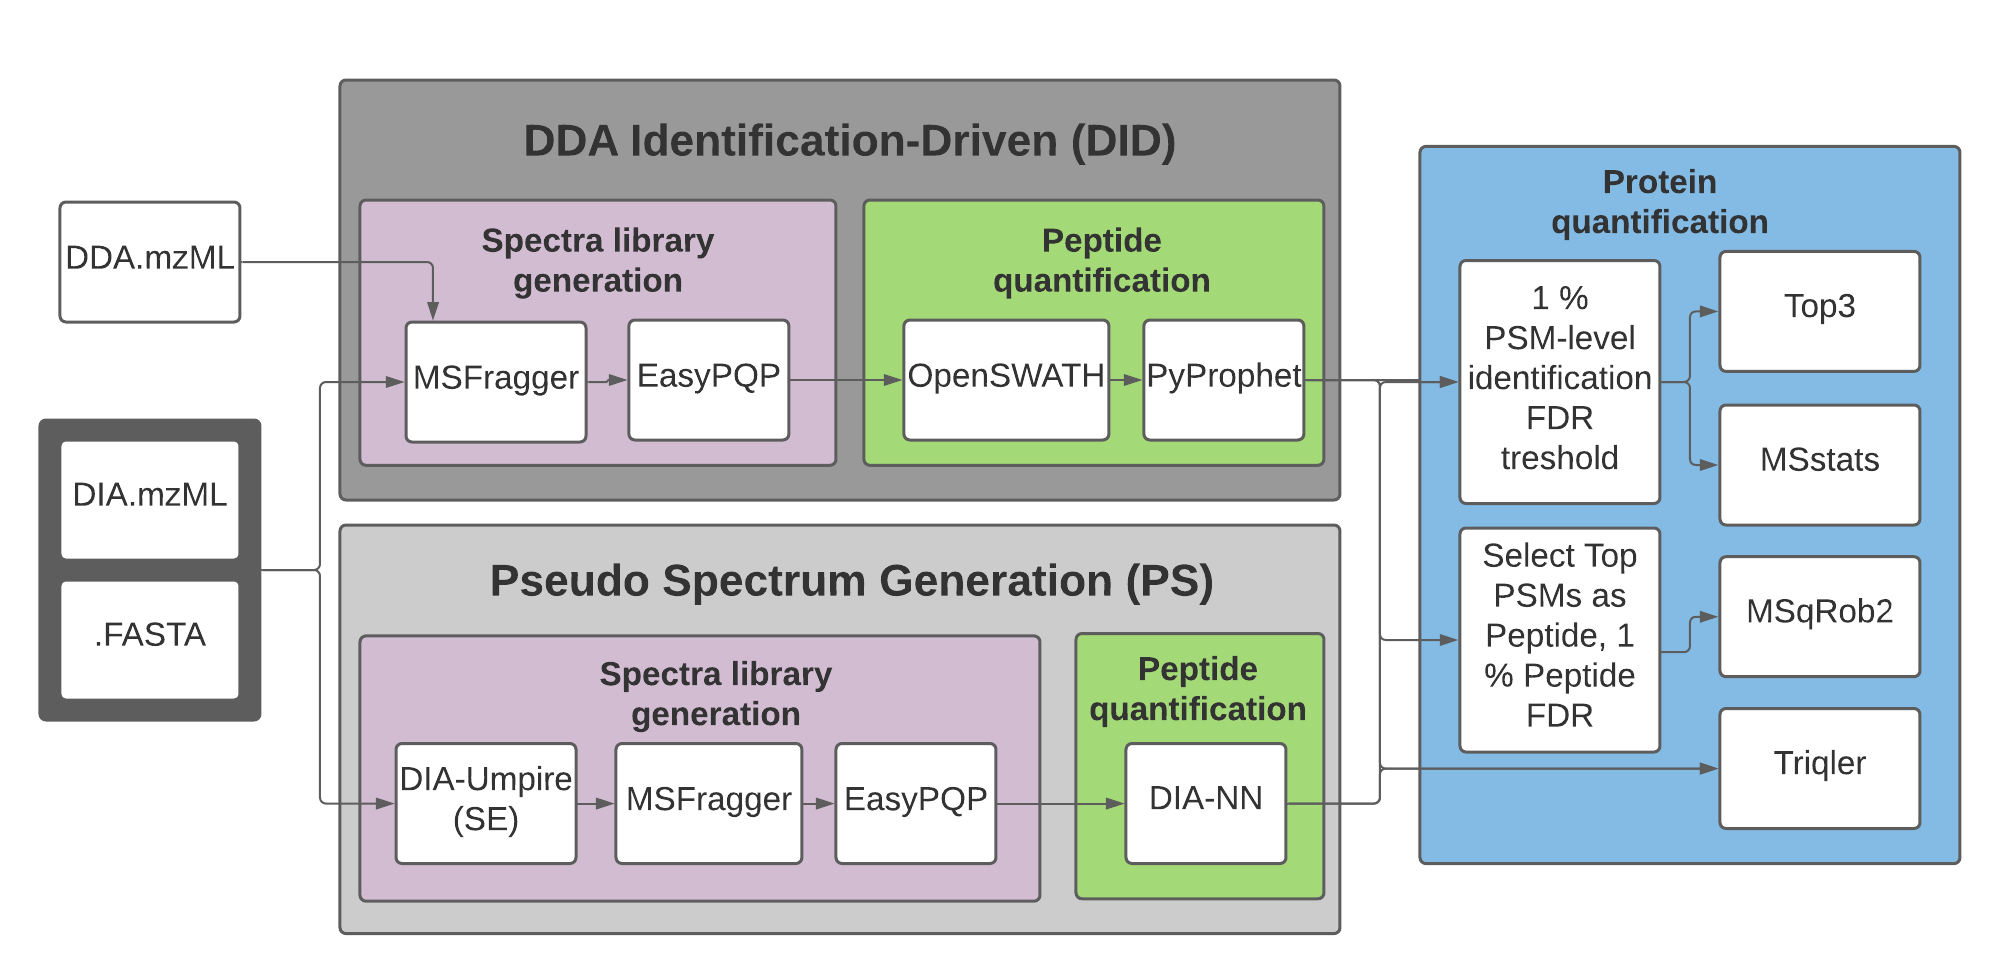
\includegraphics[width=1.1\linewidth]{../../result/report_plots/DIA_benchmark_truncated.png} 
    \end{tabular}

        \caption{{\bf The spectrum-library matching (SL) and pseudo spectrum workflow pipelines (PS).} For the various pipelines DIA-Umpire(SE), MSFragger and EasyPQP is run from Fragpipe (\protect\url{https://fragpipe.nesvilab.org/}).}
      \label{fig:flowchart}
\end{figure}



\subsubsection*{Spectral library matching (SL)}

For the Spectral Library (SL) workflow we searched the LFQBench provided DDA runs with MSFragger\cite{kong2017msfragger} with a precursor mass tolerance of [-20, 20] ppms, fragment tolerance of 20 ppms, and constructed a spectral library with EasyPQP \cite{easypqp} to from the DDA-search results using a PSM-level FDR treshold of 0.01, peptide-level FDR treshold of 0.01 and protein-level FDR treshold of 0.01 (default settings). Decoys for the spectral library was generated with OpenSwathDecoyGenerator with pseudo-reverse method. The spectral library was subsequently matched to the DIA data with the OpenSwath Workflow and  PyProphet\cite{teleman2015diana} was used for computing false discovery rate (m\_score) for the peptide quantification. This resulted in a set of detected peptides together with their assesed peptide identification accuracies and abundance estimates.

%Two approaches were used for spectra library generation: DDA acquisition-based spectral library generation and Prosit-based spectral library generation using only .fasta file \cite{searle2020generating}. 
%For Prosit-based spectral library generation, the FASTA file was converted to Prosit input format using encyclopeDIA converter. Prosit\_2020\_intensity\_cid model was used as an intensity prediction model and Prosit\_2019\_irt was used as iRT prediction model.  \todo{I am confused, are there three different workflows?[ANSWER: Not at this moment, buy my ambition is to at some point get the encyclopeDIA going, perhaps we can skip this?]}


\subsubsection*{Pseudo Spectrum generation (PS)}

For the PS workflow we also used the fragpipe software, employing DIA-Umpire to extract pseudo-spectra from the DIA data. The pseudo-spectra were subsequently searched using using MSFragger with a precursor mass tolerance of -20, 20] ppms, fragment tolerance of 20 ppms, and allowing for oxidation on methionine and protein N-terminus modifier as variable modifications. \todo{What is the N-terminus protein modifier and N-terminus peptide modifier?} A spectral library was build from the resulting PSMs at the default PSM-level treshold of 0.01 using easyPQP. DIA-NN was used for peptide quantifications, a method that uses a built-in custom implementation of the mProphet algorithm to compute $q$~values \cite{reiter2011mprophet, demichev2020dia}.
 
%For the PS workflow we also used the fragpipe software, employing DIA-Umpire to extract pseudo-spectra from the DIA data. The pseudo-spectra were subsequently searched using using MSFragger with a precursor mass tolerance of -20, 20] ppms, fragment tolerance of 20 ppms, and allowing for [M,[\^{}] variable modifications (M - oxidation on methionine and \^{} is a terminus modifier for protein N-terminal). \todo{This is confusing. Spell out what it means. Do you look for N-term methionines, or is it something different?} A spectral library was build from the resulting PSMs at the default PSM-level treshold of 0.01 using easyPQP. DIA-NN was used for peptide quantifications, a method that uses a built-in custom implementation of the mProphet algorithm to compute $q$~values \cite{reiter2011mprophet, demichev2020dia}.
 
 %The DIA-NN uses a built-in mProphet algorithm with decoy precursors to compute the $q$~values. \cite{reiter2011mprophet} \cite{demichev2020dia}. 

% VARIABLE MODIFICATION 
% https://github-wiki-see.page/m/Nesvilab/MSFragger/wiki/Setting-the-Parameters 

%\subsection*{Database searching}
%For both workflow we matched spectra and pseudo-spectra with MSFragger with parameters: [check parameters], and used peptide-prophet for statistical validation was performed by peptide prophet and protein prophet.


\subsection*{Protein summarization}

The peptide quantities was summarized to proteins using the average of the three most intense peptides (We call it Top3), MSstats, MSqRobSum and Triqler for both the spectral library and the pseudo-spectra pipelines. 

\subsubsection*{Top3}

We implemented a short script that for each protein selected the average of the 3 most abundant peptides for each protein and sample if there were 2 or more peptide intensities available. 

% res = triq_run.groupby("proteins")["intensity"].apply(lambda x: x.nlargest(3).mean() if len(x.nlargest(3)) >= 2 else np.nan).reset_index()

%We implemented a short script that for each protein selected the three, on average, most abundant peptides across the conditions and summarized their protein quantities.

\subsubsection*{MsStats}

We installed MSstats version 3.18.5 using R/Bioconductor (available at \url{https://www.bioconductor.org/packages/release/bioc/html/MSstats.html}). MSstats was run using the MSstats command \texttt{dataProcess} without any peptide och m\_score filtering on the input data. The significance testing between conditions was performed using the MSstats function \texttt{groupComparison}.  

\subsubsection*{MSqRobSum}

We installed MSqRobSum version 0.9 using R/Bioconductor (available at \url{https://github.com/statOmics/MSqRobSum}). MsqRobSum was run using the MSqRobSum command \texttt{msqrobsum}, mode was set to \texttt{msqrobsum}, contrast was set to \texttt{condition} and \texttt{group\_vars} was set to the species human, yeast and \textit{E.Coli}. The \texttt{formulas} variables was set to \texttt{c(expression ~ (1|condition) + (1|sample) + (1|feature), expression ~ (1|condition))}. This means that the two models $y_{st} = \beta_0 + \beta_{condition} + \beta_{sample} + \beta_{feature} + \epsilon$ and $y_{st} = \beta_0 + \beta_{condition} + \epsilon$ was specified for MSqRobSum analysis. This setup makes sure that if the fist models fails, the second models is tried. 

%We downloded MSqRobSum version 0.9 from \url{FIXME}.

\subsubsection*{Triqler}

The code for Triqler is kept at \url{https://github.com/statisticalbiotechnology/triqler}. We used Triqler v0.6.1 for the tests described in this paper. Triqler was run with \texttt{fold\_change\_eval} parameter between 0 and 2.00 with 0.04 increments.

\subsubsection*{Multiple Hypothesis Correction}
There was a slight difference in some of the benchmarking metrics, as the multiple test correction is performed with $q$~value for Triqler and Top3, while MsStats and MSqRobSum uses Benjamini-Hochberger \cite{benjamini1995controlling} corrections. The $q$~value approach aims to give a unbiased estimator of FDR, while the Benjamini-Hochberger approach estimates the upper bound of the FDR. As a consequens, the statistics from MsStats and MSqRobSum should be slightly more conservative \cite{korthauer2019practical}.

%For the OSW-pipeline the recommended pipeline consisting of running TRIC feature alignment was used before MSstats and msqrob conversion \todo{If I recall correctly non of the features was actually aligned, but I will rerun the computations to double check}. For all other data we did not use TRIC aligned peptide data. 


\section*{Results}



\subsection*{Validations of properties of DIA peptide abundance}

Triqler was designed for handling DDA data, and it was hence essential to validate that some of the assumptions Triqler makes about peptide abundance data, also are true for DIA datasets.
We hence downloaded the LFQBench dataset and processed it with two differnt piplenes, and investigated the properties of the reported pepide abundances. DIA data is known to encompass a larger dynamic range than DDA data \citation{bilbao2015processing}. This could affect one of Triqles assumptions, that the noise structure is mainly multiplicative, i.e. that the standard deviation within a sample group is proportional to its mean. When investigating all the peptide abundance measurements at a 1\% identification FDR from the TripleTOF6600 section of the LFQBench dataset, we found a relatively linear relation between standard deviation and mean (Supplementary Figure \ref{fig:assumptions}A). Further, Triqler assumes that the missing peptide abundance values follow a censored normal distribution, which is also roughly fullfilled by DIA data (See Supplementary Figure \ref{fig:assumptions}B).


\subsection*{Summarizing to protein concentrations}

We wanted to compare the performance of Triqler to that of other protein summarization methods. An inherent problem when comparing different protein summarization softwares is that the performance is affected by which protein inference structure is used, in a data set dependent manner \cite{serang2012recognizing}. For example, when reporting number of differentially abundant proteins in data sets from mixtures from whole-cell extracts, a protein inference scheme that infer any protein contain a detected peptide will report more differentially abundant proteins than more restrictive scheme that just report a parsimonous set of proteins. For such data sets there is no mechanisms restrictive mechanism detecting situations where non-present proteoforms are reported as long as they are part of and reported with protein abundance rates compatible to the right proteome. To elaviate, or at least minimize, this problem from our comparison, we restricted the searched FASTA files by removing proteins with shared peptides. This operation stived to 
give a fairer comparison of protein summarization regardless of the protein inference method.

Given the peptide abundances derived from the SL and PS workflows, we could now compare the performance of Triqler to the one of msStats, msSqRobSum and Top-3. Here we selected to run Triqler with a lower bound estimate as described in The\&K\"{a}ll \cite{the2021triqler}, which ended up as 0.76 for the spectral library data, and 0.52 for the pseudo-spectra enabled data.

\subsubsection*{Fold change distributions}

To get an overview of the results of the methods we first made histograms of the reported protein level fold-changes as reported by the compared methods in Figure \ref{fig:fc_histogram}. For the these plots we removed all error assements on protein-level. We observe that Triqler and Top3 has less bias than MSstats and MSqRobSum, by seeing that the apex of the distributions are centered more closely to the true values. MSqRobSum report a very large number of proteins at a fold-change of zero. These peaks all have a false discovery rate of 1.00, and would normally be filtered away by tresholding.

%FIXME: Remove this, Figure \ref{fig:fc_histogram_again}.

\begin{figure}[hbt]
    \centering
    %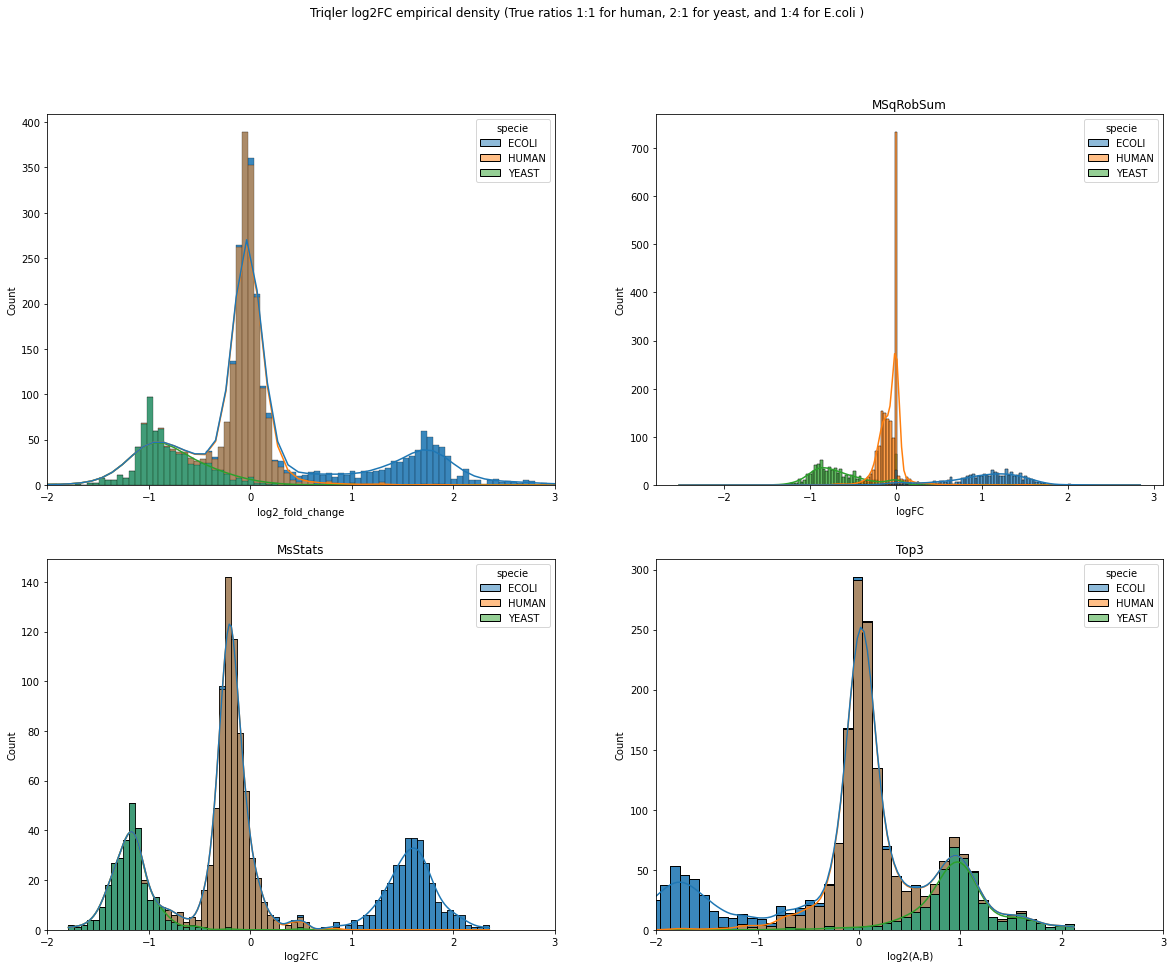
\includegraphics[width=16cm]{../../result/2021-08-13_docs_plots/intensity_plot.png}
    \begin{tabular}{lclc}
	    A & 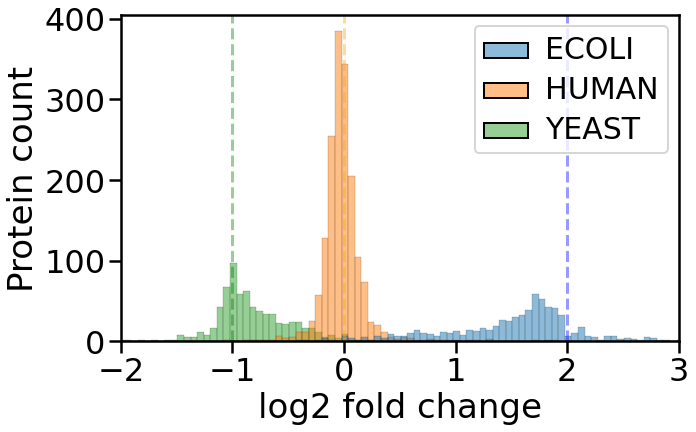
\includegraphics[width=0.4\linewidth]{../../result/report_plots/osw_triqler_intensity.png} & 
	    B & 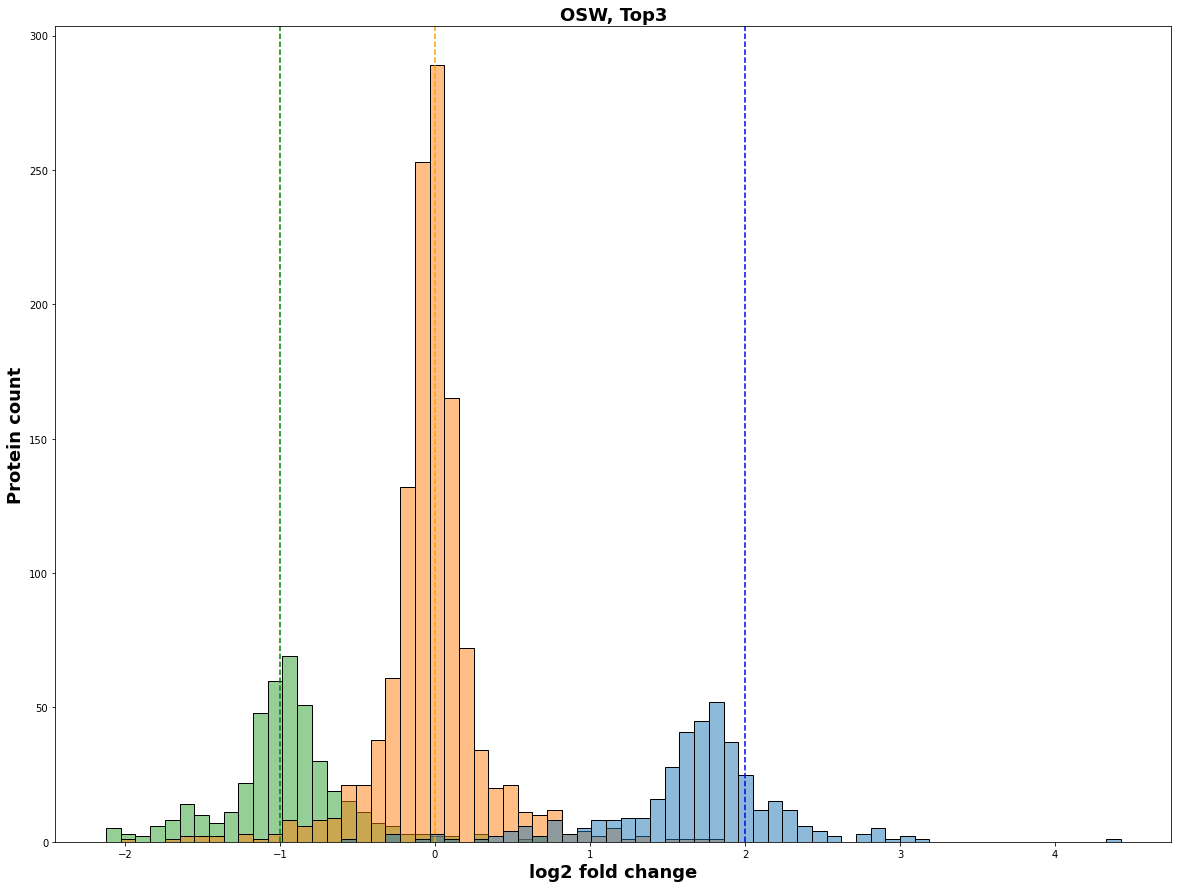
\includegraphics[width=0.4\linewidth]{../../result/report_plots/osw_top3_intensity.png} \\ 
	    C & 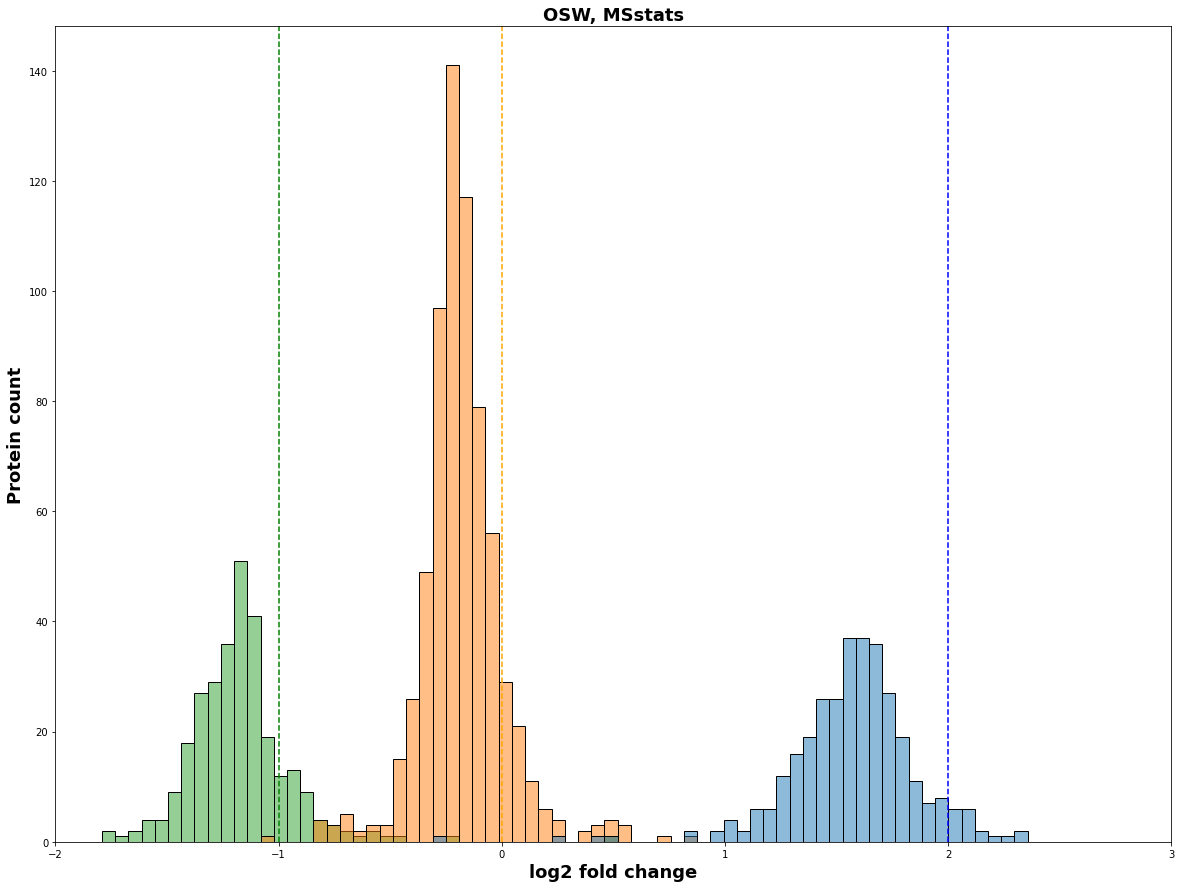
\includegraphics[width=0.4\linewidth]{../../result/report_plots/osw_msstats_intensity.png} & 
	    D & 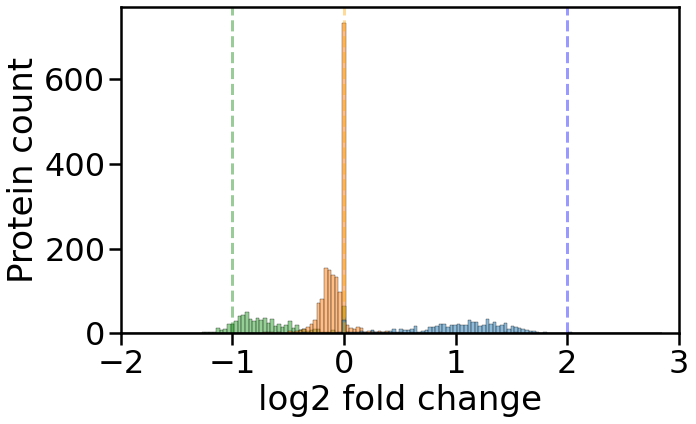
\includegraphics[width=0.4\linewidth]{../../result/report_plots/osw_msqrobsum_intensity.png} \\ 
        %A & 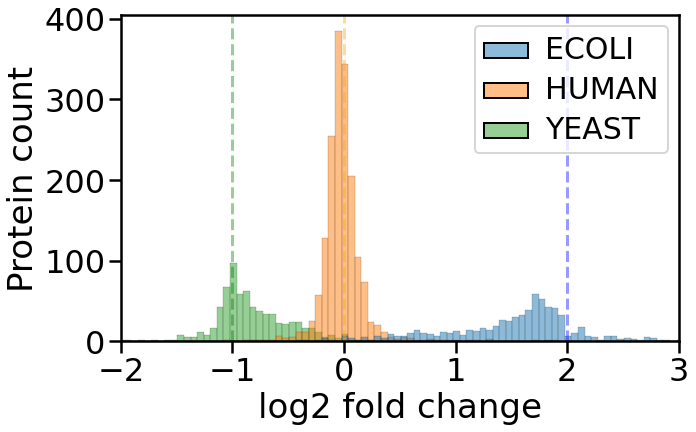
\includegraphics[width=0.4\linewidth]{../../result/report_plots/osw_triqler_intensity.png} & 
        %E & 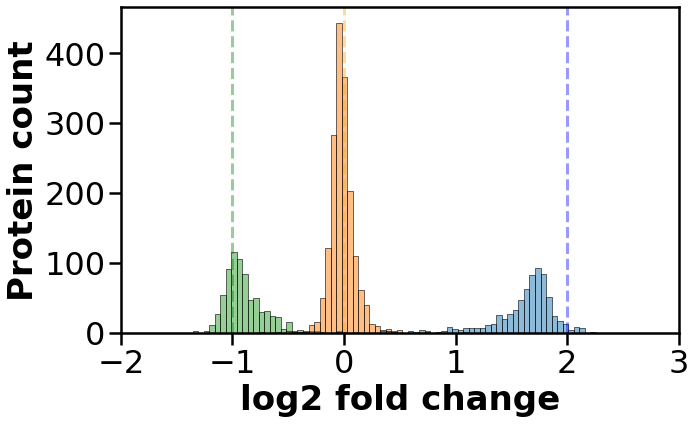
\includegraphics[width=0.4\linewidth]{../../result/report_plots/diann_triqler_intensity.png} \\ 
        %B & 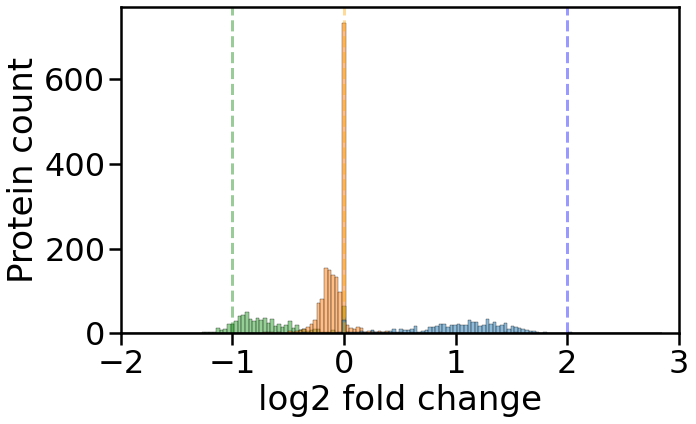
\includegraphics[width=0.4\linewidth]{../../result/report_plots/osw_msqrobsum_intensity.png} & 
        %F & 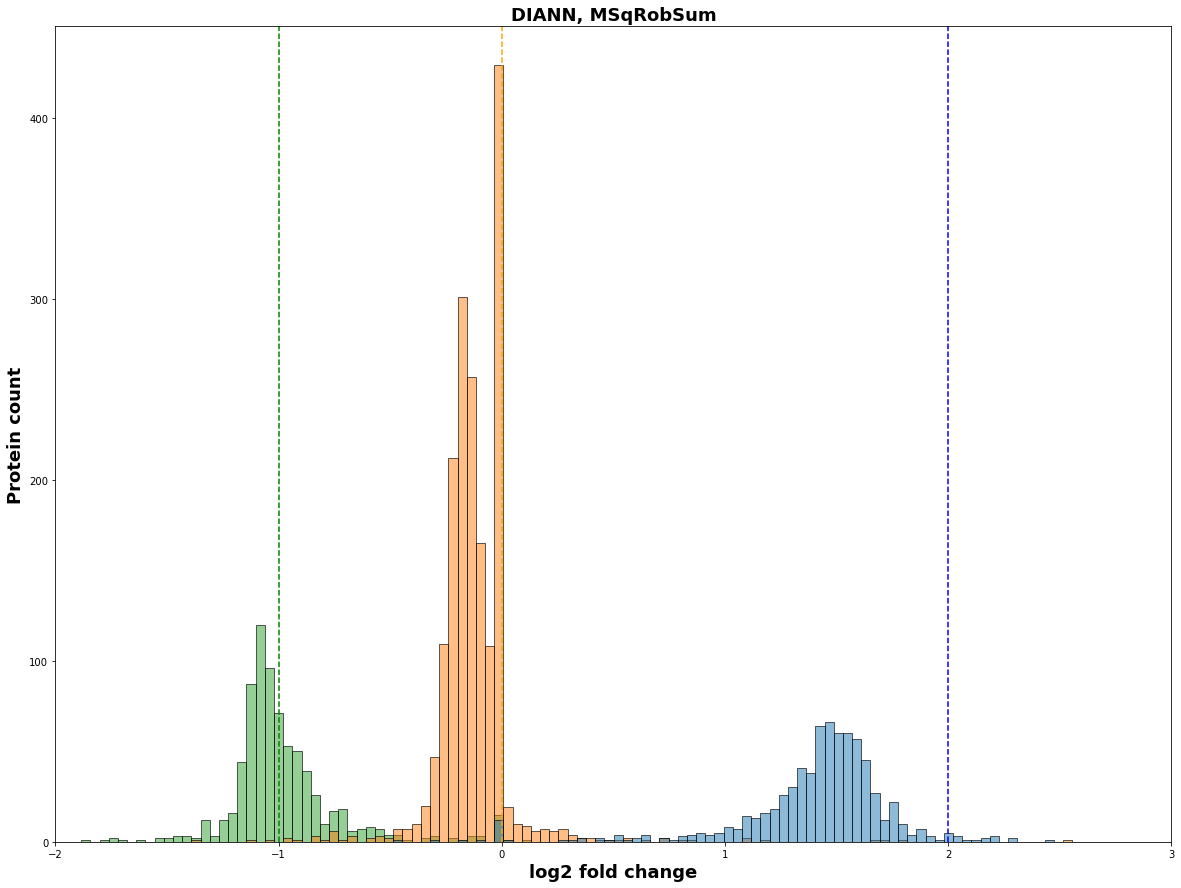
\includegraphics[width=0.4\linewidth]{../../result/report_plots/diann_msqrobsum_intensity.png} \\ 
        %C & 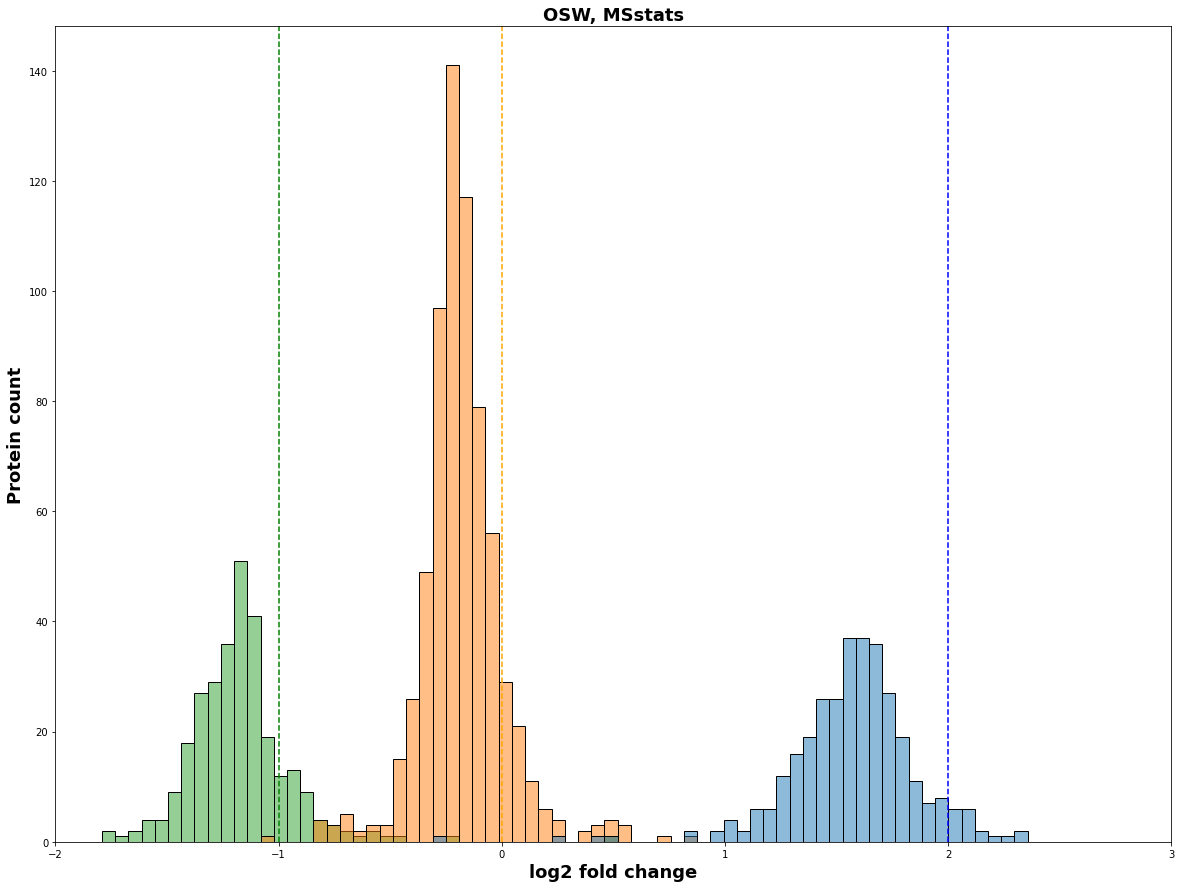
\includegraphics[width=0.4\linewidth]{../../result/report_plots/osw_msstats_intensity.png} & 
        %G & 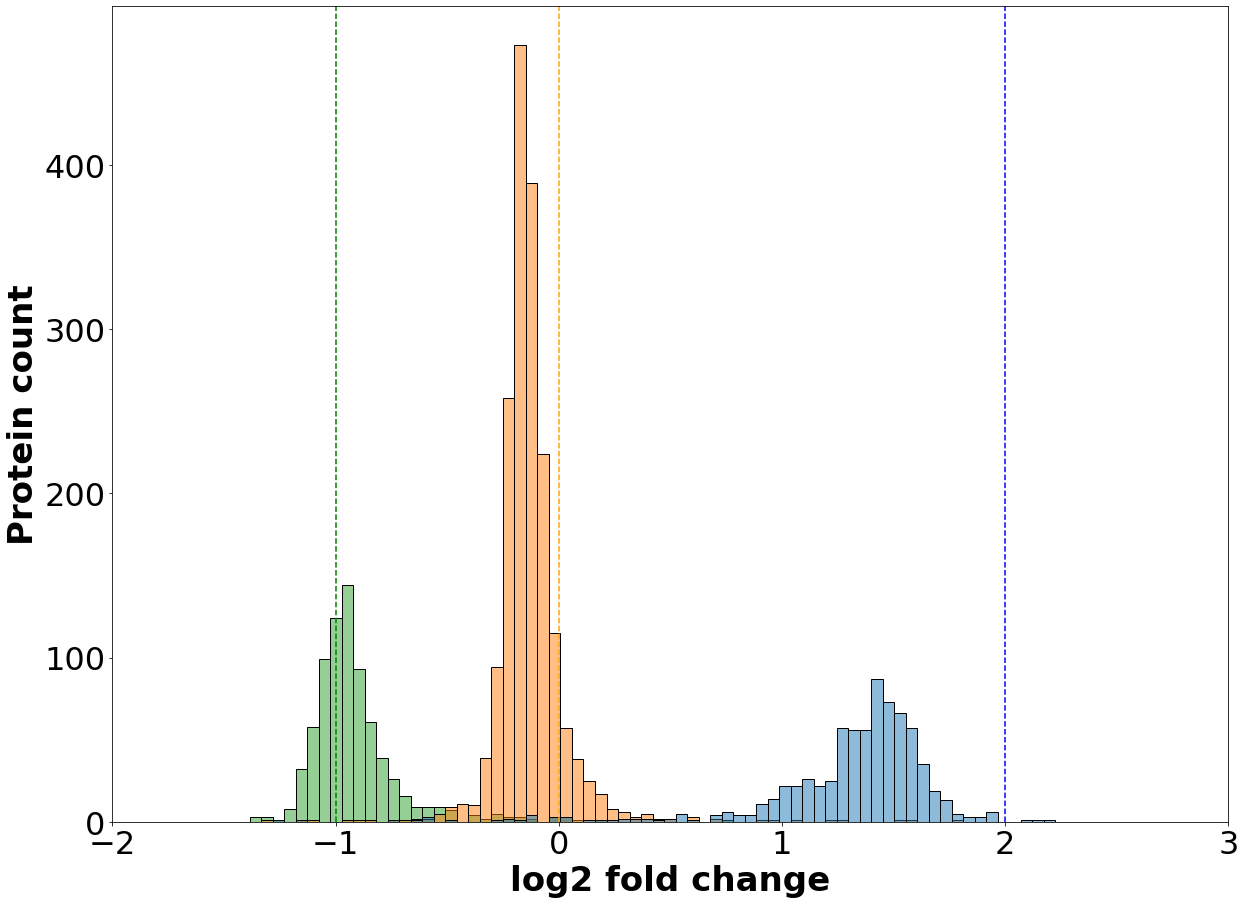
\includegraphics[width=0.4\linewidth]{../../result/report_plots/diann_msstats_intensity.png} \\ 
        %D & 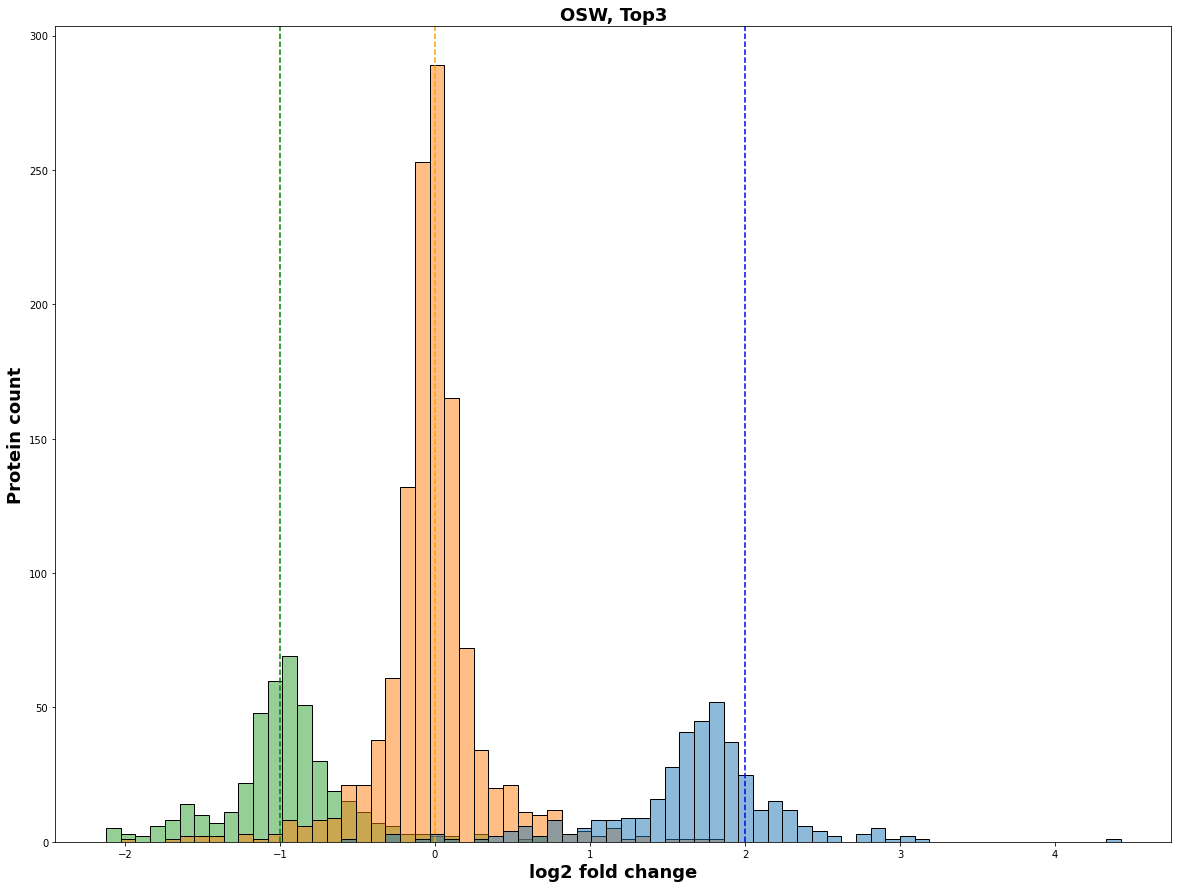
\includegraphics[width=0.4\linewidth]{../../result/report_plots/osw_top3_intensity.png} &
        %H & 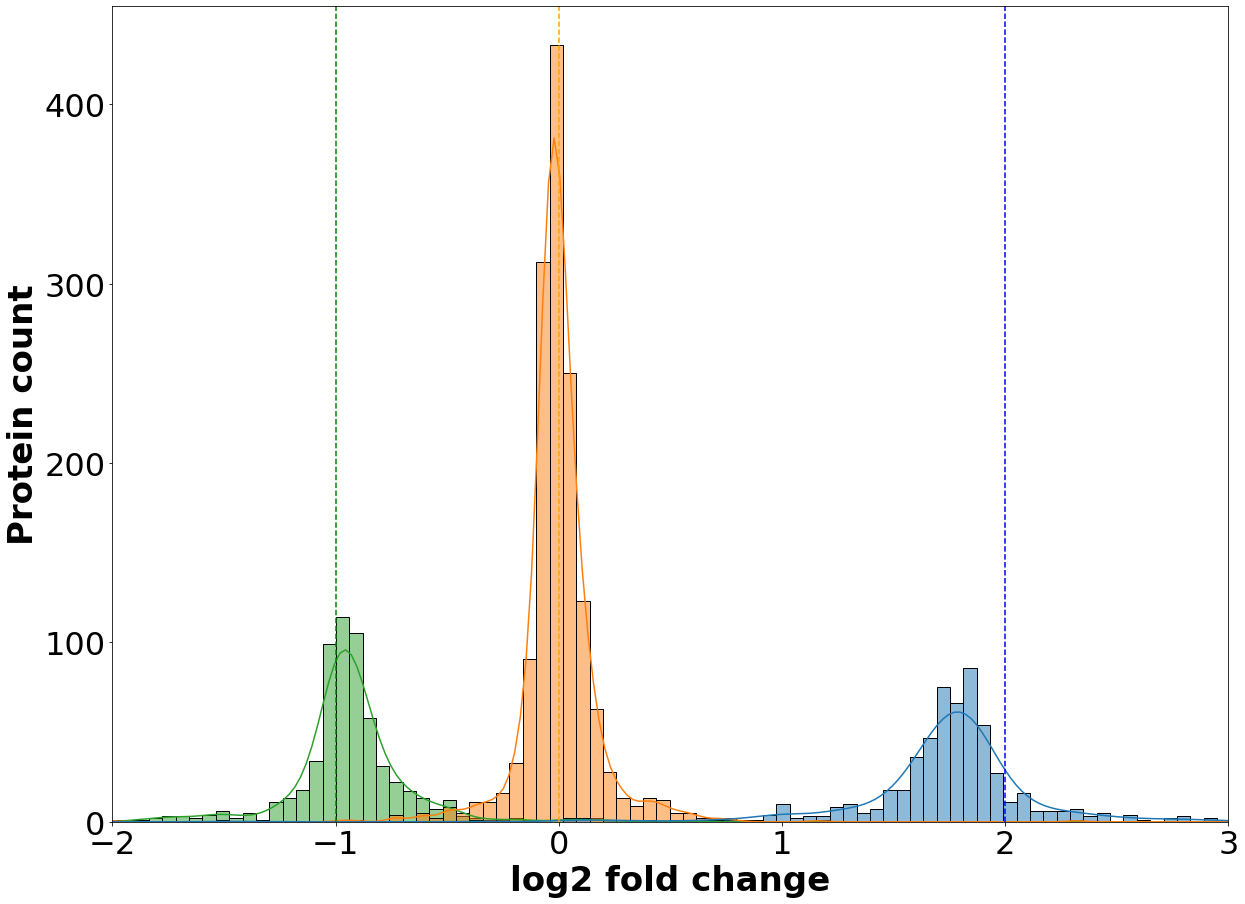
\includegraphics[width=0.4\linewidth]{../../result/report_plots/diann_top3_intensity.png} 
    \end{tabular}
    \todo[inline]{Try to find and explanation of the large difference in nuRmber of reported proteins for e.g. the C and G subplot.}
    \caption{{\bf Comparison of reported fold change distributions.} We used peptide data from SL and (A) Triqler, (B) Top3, (C) MSstats, and (D) MSqRobSum. The dashed lines indicates the true log2-fold change ratio between a specie and HeLa samples. We note that the empirical densities of the protein count are less biased for Triqler and Top3 than MSstats and MSqRobSum by observing that the apex of the distribution is closer to the dashed line. (D) MSqRobSum report a large log2 fold change bin at 0. A majority of these valued have been filtered away using a tresholding procedure because the reported false discovery rate for the difference between groups was 1.0 for most values in this bin. \label{fig:fc_histogram}}
\end{figure}

\subsubsection*{Comparison of ability to discriminate differentially from equally abundant proteins}

The LFQBench set contain varying concentrations of {\em E. Coli} and Yeast concentrations in a background of HeLa-cells. As a first test of performance we hence compared the methods' ability to infer the differentially abundant {\em E. Coli} and Yeast protein as a function of the number of false positives from the HeLa-background, when varying the reported significance treshold (Figure \ref{fig:diff_vs_hela}). Overall, it seems like Triqler reports more true differential abundat protein for every false differential abundant protein for both spectral library matching and pseudo-spectrum methods. Surprisingly, Top3 performs has more true differentially abundant proteins for every false protein than MSstat and MSqRobSum. 



\begin{figure}[hbt]
    \centering
    \begin{tabular}{lclc} 
%        A & 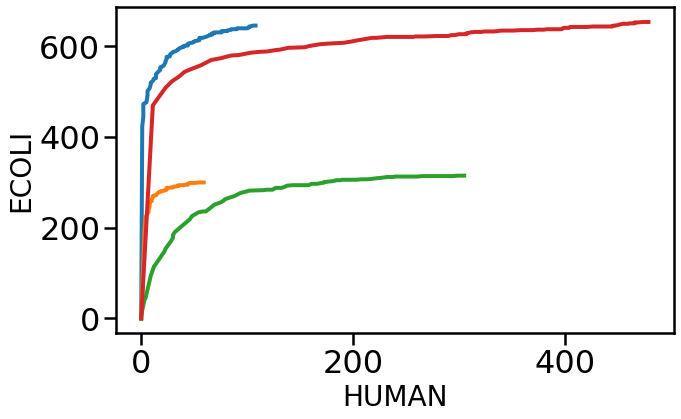
\includegraphics[width=0.4\linewidth]{../../result/report_plots/osw_de_human_vs_ecoli.png} & 
%        C & 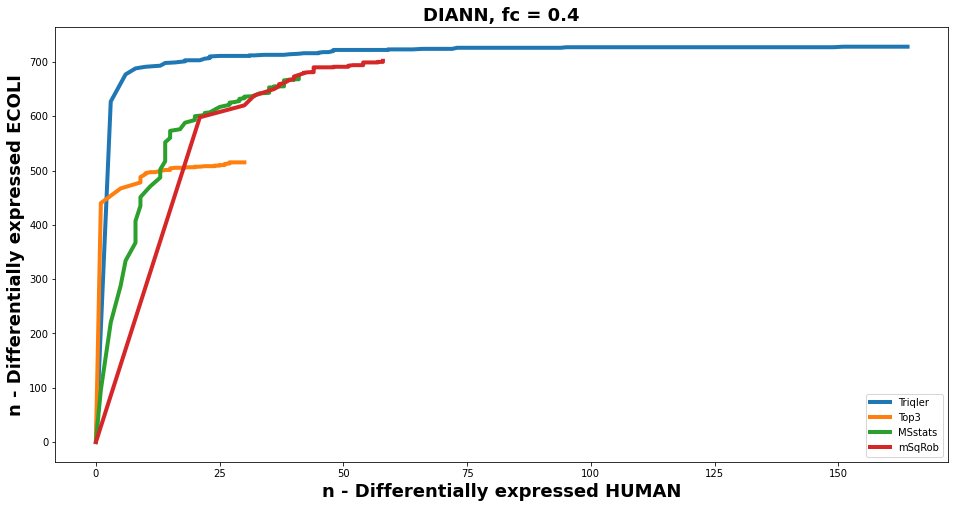
\includegraphics[width=0.4\linewidth]{../../result/report_plots/diann_de_human_vs_ecoli.png} \\ 
%        B & 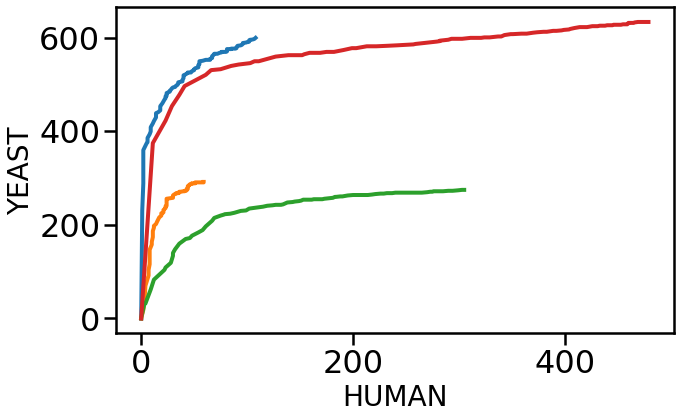
\includegraphics[width=0.4\linewidth]{../../result/report_plots/osw_de_human_vs_yeast.png} & 
%        D & 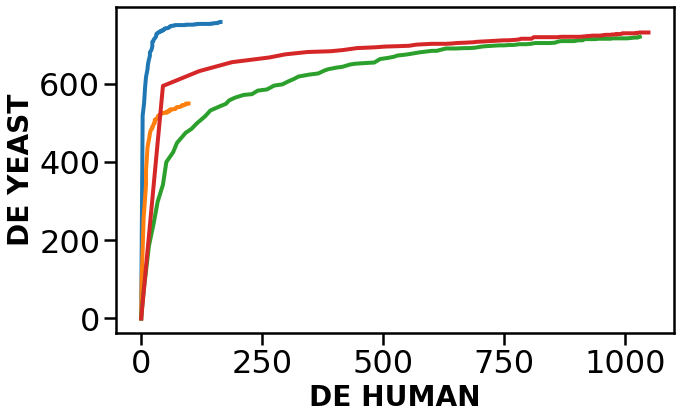
\includegraphics[width=0.4\linewidth]{../../result/report_plots/diann_de_human_vs_yeast.png} 
        A & 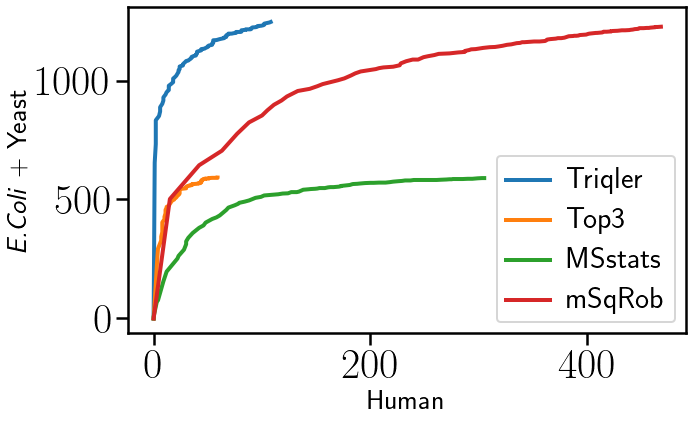
\includegraphics[width=0.45\linewidth]{../../result/report_plots/osw_de_human_vs_ecoli_and_yeast.png} & 
        B & 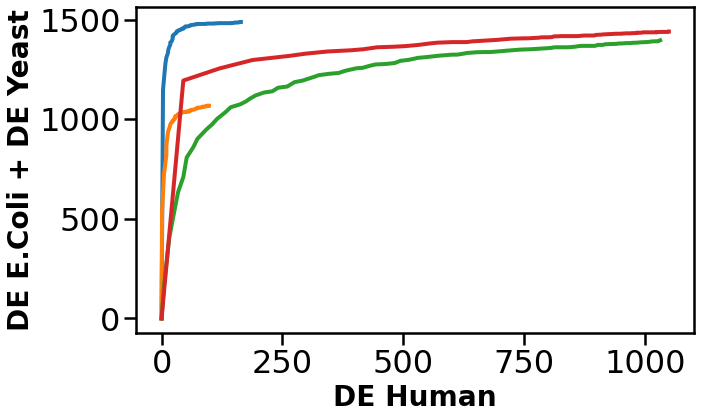
\includegraphics[width=0.45\linewidth]{../../result/report_plots/diann_de_human_vs_ecoli_and_yeast.png} \\ 

    \end{tabular}
    %\todo[inline]{Merge the plots so ythat you report the number of differentialy abundant yeast+ecoli proteins as a function of human proteins proteins. "E. coli" should be written in italics.
    %}   
    \caption{{\bf Comparison of ability to differentiate differentially abundant proteins} We plotted the number of reported differentially abundant  {\em E. Coli} and Yeast proteins as a function of number of proteins from the HeLa background when sorting according to significance for (A) DDA generated spectral libraries and (B) DIA-Umpire geneated Pseudo spectra. For the test we selected a fold-change treshold of 0.4 for Triqler, because it is the rounded lower bound for fold-change computed by Triqler (Supplement Figure \ref{fig:ability_to_differentiate_differentially_abundant_specie_vs_hela} shows differential abundance for each specie). \label{fig:diff_vs_hela}}
\end{figure}



\subsubsection*{Differential abundance}

We also report the amount of differentially abundant proteins in Figure \ref{fig:da_lineplot} to show the performance of of the compared methods. We compare two-sided differential abundance since Triqler computes two-sided fold change. A fold-change treshold of 0.4 has been applied to Triqler, but not Top3, MSstats or MSqRobSum. This should give an disadvantage to Triqler. We observe that Triqler and MSqRobSum are the best performing protein quantification methods for {\em E. Coli} and Yeast in both spectral library matching and pseudo-spectrum workflows. We observe that MSqRobSum and MSstats report far more differentially abundant human proteins than Triqler and Top3. These are false hits.   

\begin{figure}[hbt]
    \centering
    %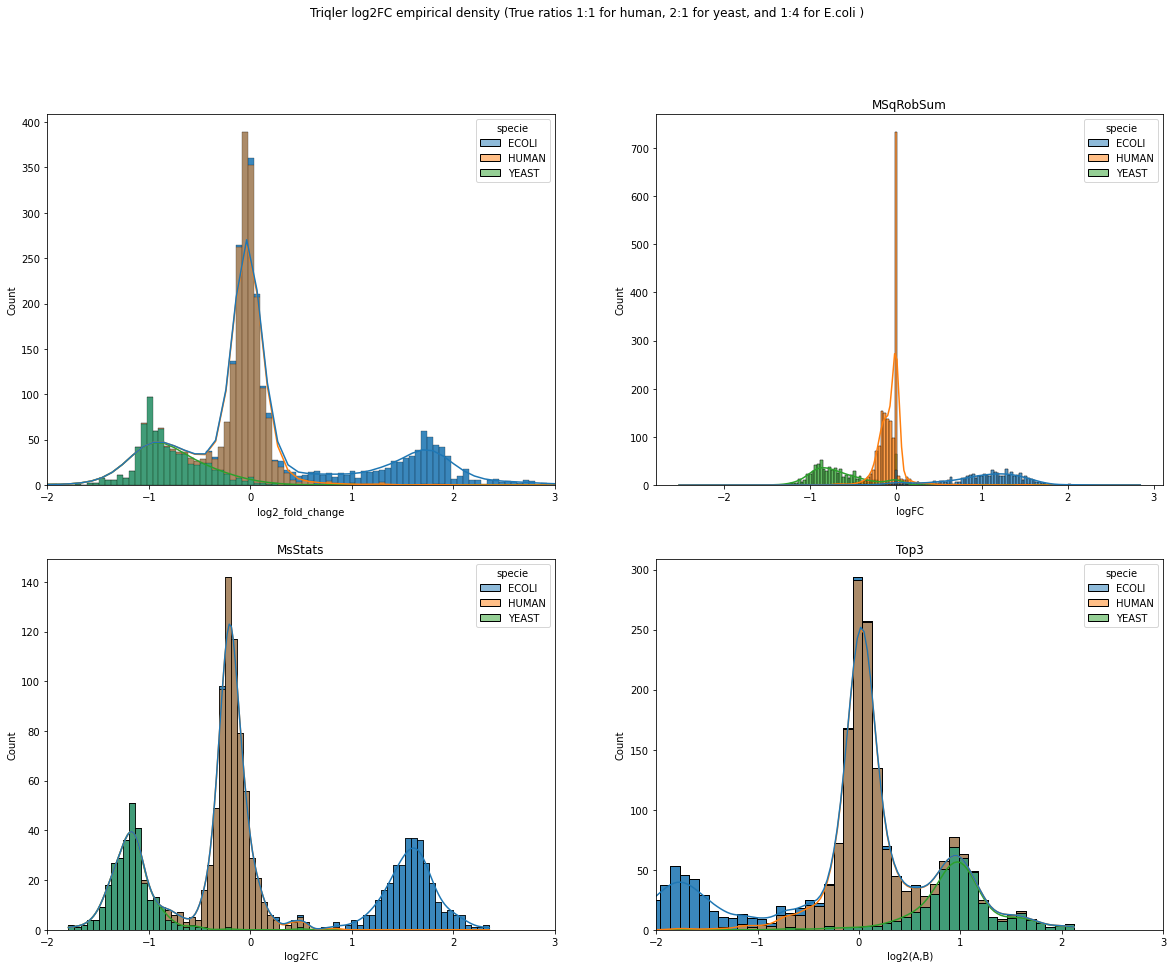
\includegraphics[width=16cm]{../../result/2021-08-13_docs_plots/intensity_plot.png}
    \begin{tabular}{lclc} 
        A & 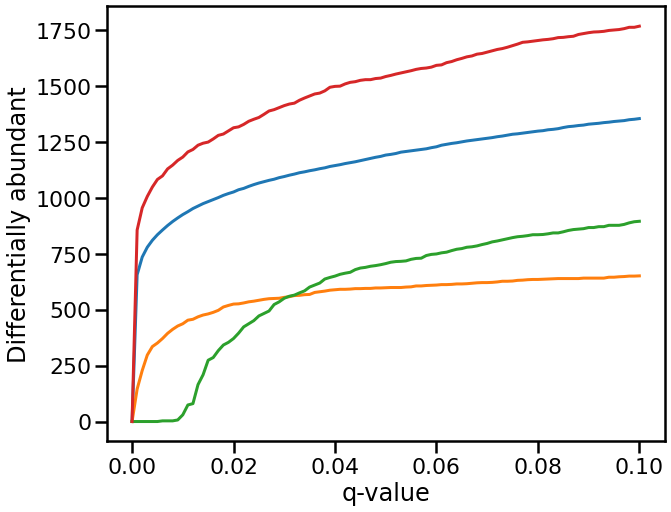
\includegraphics[width=0.4\linewidth]{../../result/report_plots/osw_de_all.png} & 
        E & 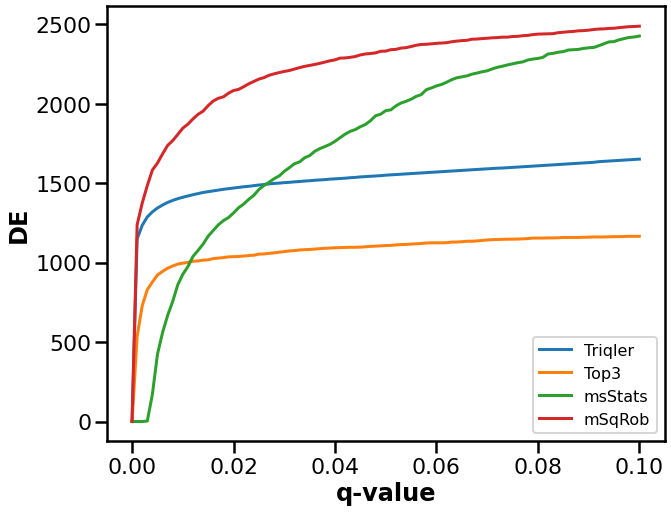
\includegraphics[width=0.4\linewidth]{../../result/report_plots/diann_de_all.png} \\ 
        B & 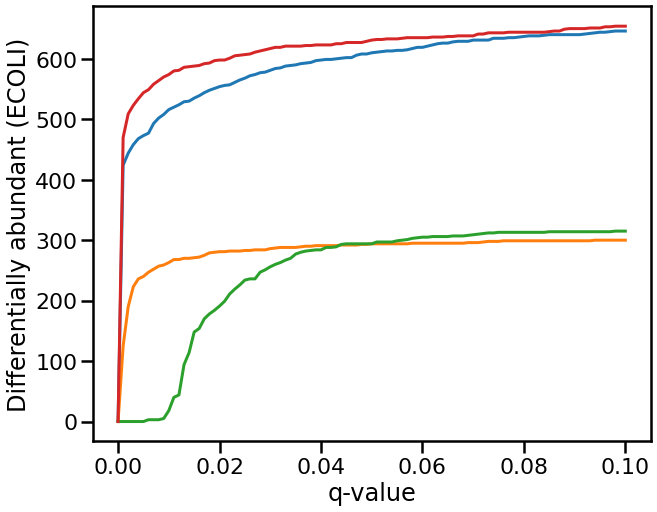
\includegraphics[width=0.4\linewidth]{../../result/report_plots/osw_de_ecoli.png} & 
        F & 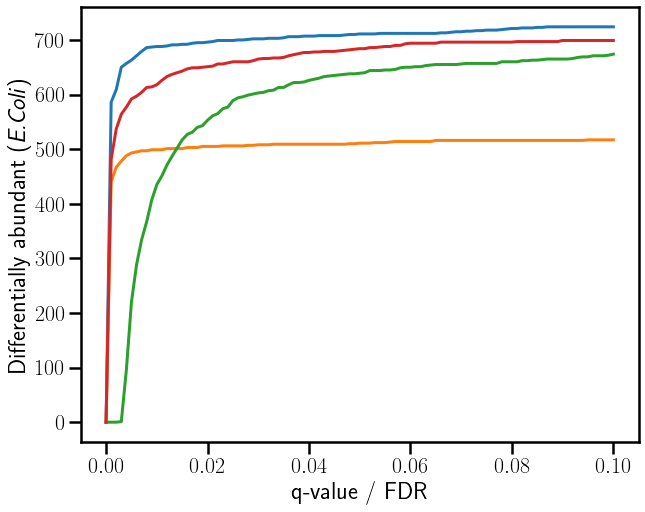
\includegraphics[width=0.4\linewidth]{../../result/report_plots/diann_de_ecoli.png} \\ 
        C & 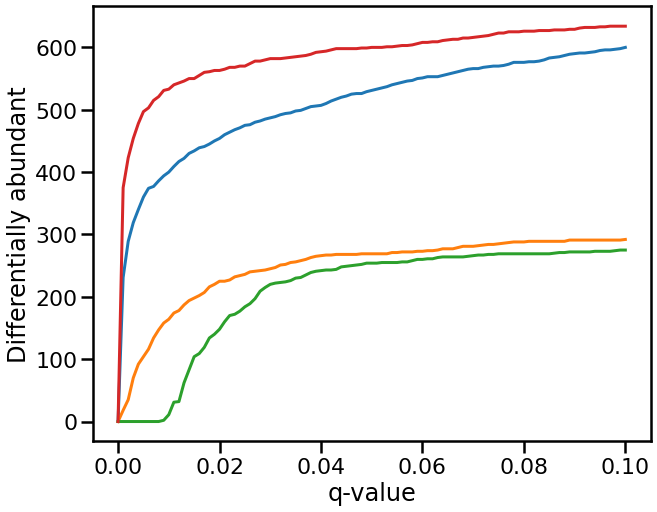
\includegraphics[width=0.4\linewidth]{../../result/report_plots/osw_de_yeast.png} & 
        G & 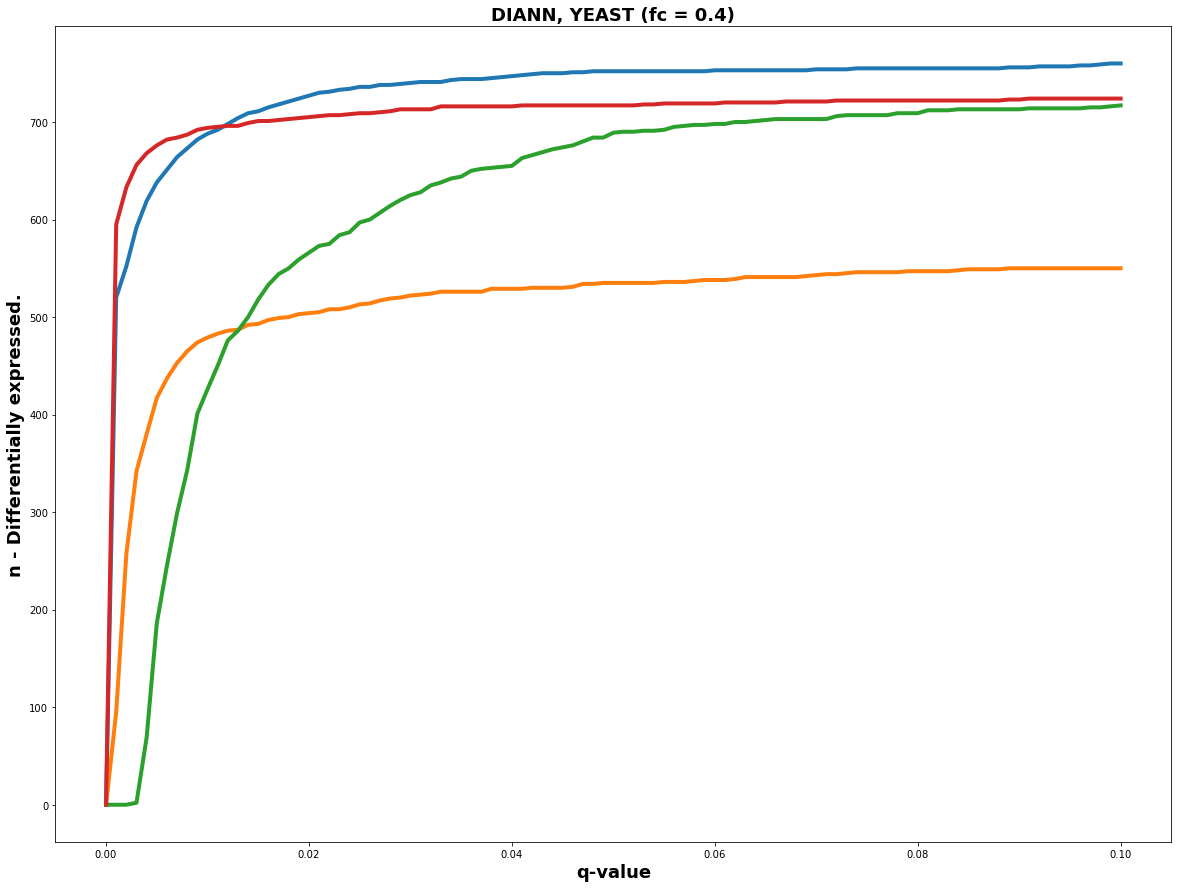
\includegraphics[width=0.4\linewidth]{../../result/report_plots/diann_de_yeast.png} \\ 
        D & 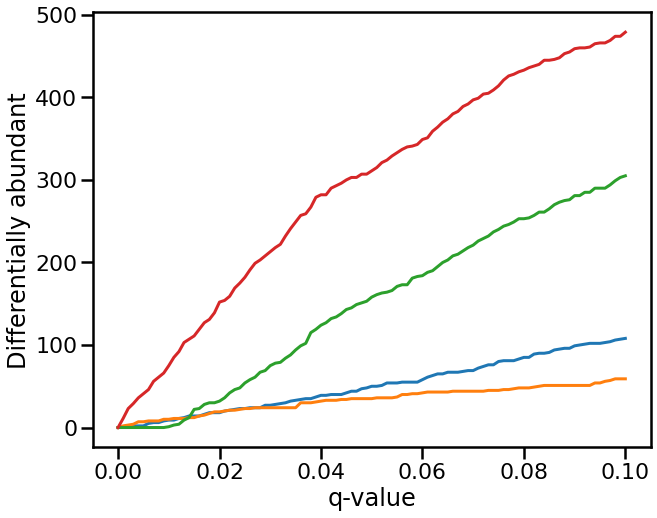
\includegraphics[width=0.4\linewidth]{../../result/report_plots/osw_de_human.png} &
        H & 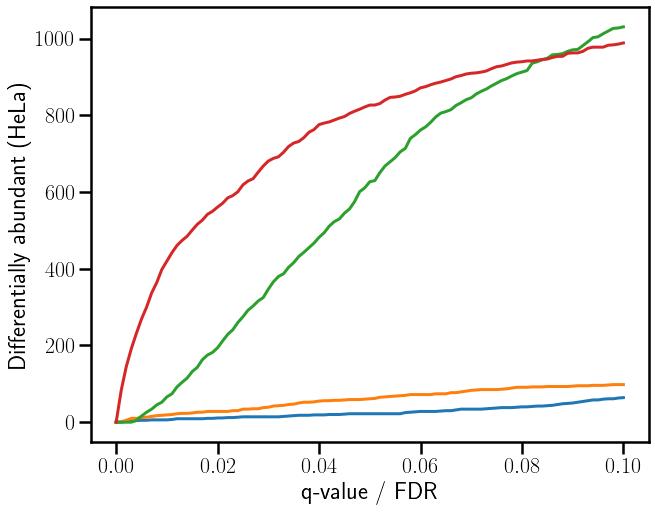
\includegraphics[width=0.4\linewidth]{../../result/report_plots/diann_de_human.png} 
    \end{tabular}
    \caption{{\bf Comparison of reported differential abundance.} Differential abundance is reported for (A-D) Spectrum library matching and (E-H) pseudo spectra workflowsf for each proteome 
    (A,E) All, (B,F) {\em E. Coli}, (C,G) Yeast, and (D,H) Human. \label{fig:da_lineplot}}
\end{figure}



\subsubsection*{Comparison of statistical calibration}

We subsequently set out to test the statistical calibration of the different summarization methods. We hence investigated the relation between the fraction of wrongly reported differential abundant proteins (i.e. the number of human proteins), and the estimated false discovery rate (See Figure \ref{fig:frac_hela_vs_fdr}). We observe that Triqler and Top3 shows a fraction of human protein that is close to the $q$~value, while MSstats and  MSqRobSum seem to have a larger amount of wrongly identified differentially abundant protein than the reported FDR. 

\begin{figure}[hbt]
    \centering
    \centering
    \begin{tabular}{lclc} 
        %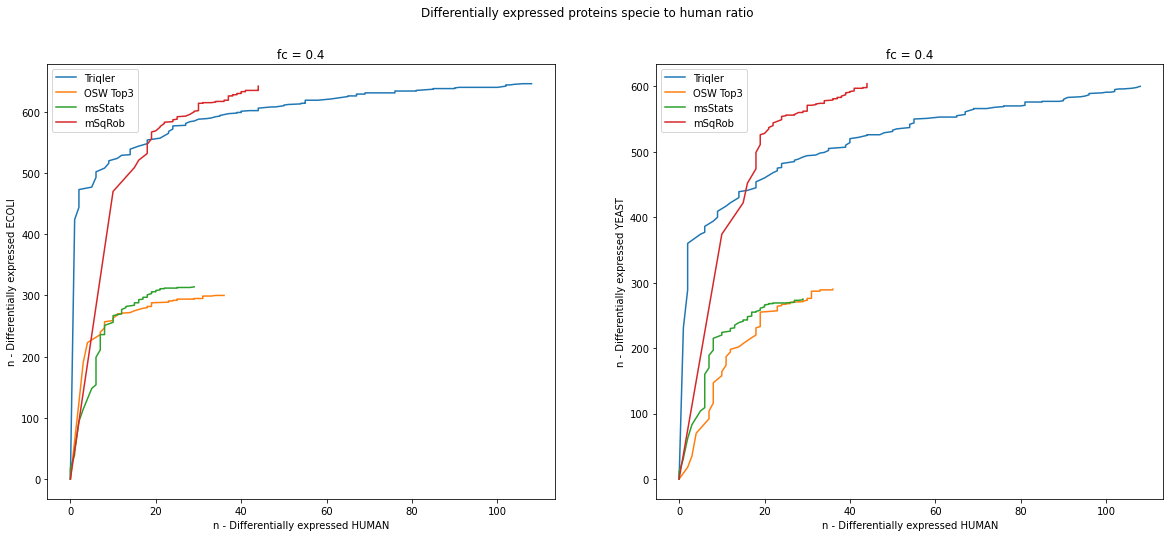
\includegraphics[width=0.3\linewidth]{../../result/report_plots/de_human_vs_de_specie.png} & 
        %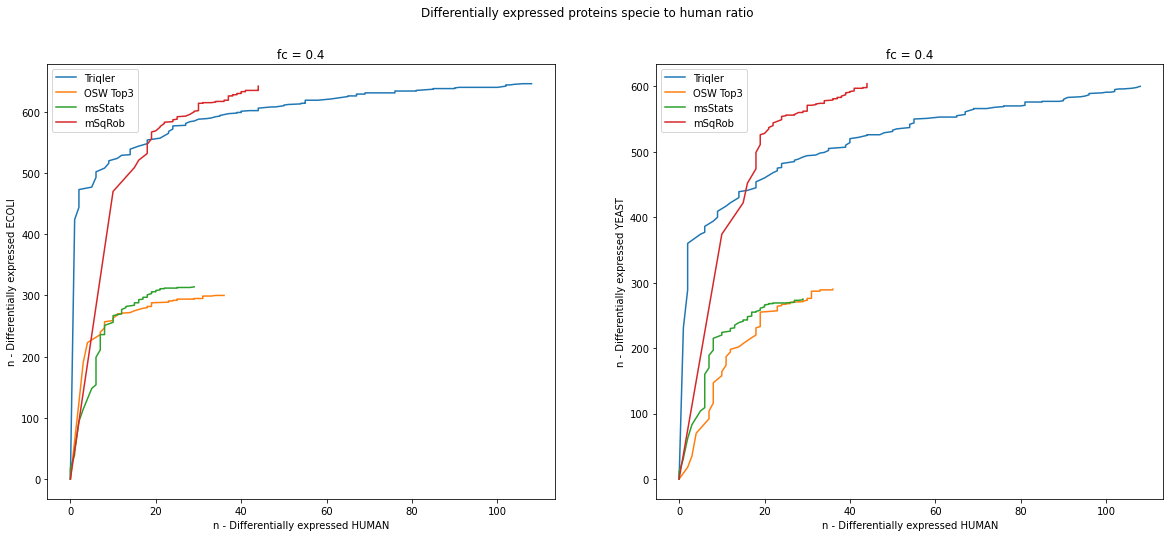
\includegraphics[width=0.3\linewidth]{../../result/report_plots/de_human_vs_de_specie.png} \\ 
        %A & B
%        A 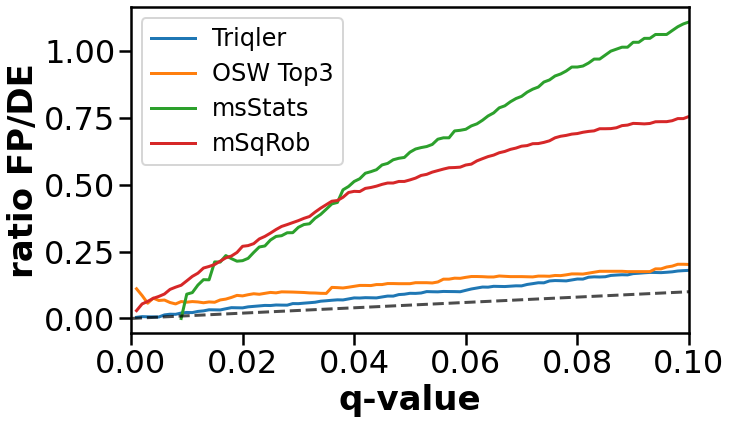
\includegraphics[width=0.5\linewidth]{../../result/report_plots/osw_FP_DE_yeast.png} & &%\includegraphics[width=0.3\linewidth]{} & 
%        D 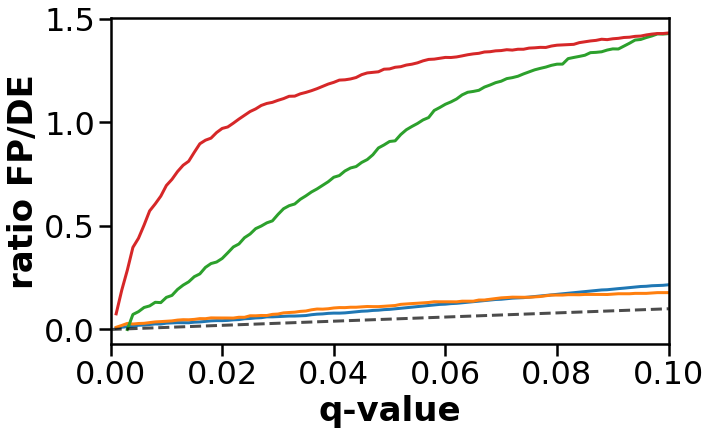
\includegraphics[width=0.5\linewidth]{../../result/report_plots/diann_FP_DE_yeast.png} & \\%\includegraphics[width=0.3\linewidth]{} \\ 
%        B 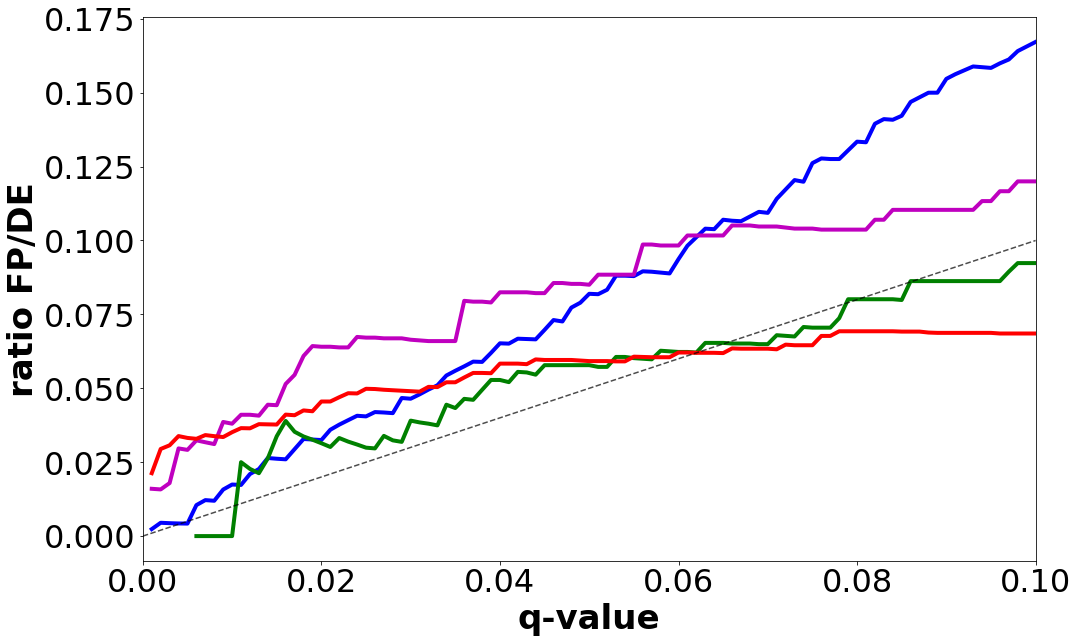
\includegraphics[width=0.5\linewidth]{../../result/report_plots/osw_FP_DE_ecoli.png} & &%\includegraphics[width=0.3\linewidth]{} & 
%        E 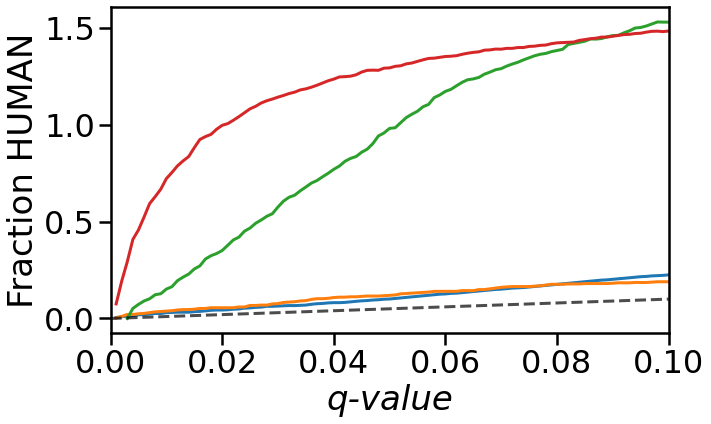
\includegraphics[width=0.5\linewidth]{../../result/report_plots/diann_FP_DE_ecoli.png} & \\%\includegraphics[width=0.3\linewidth]{} \\ 
        A 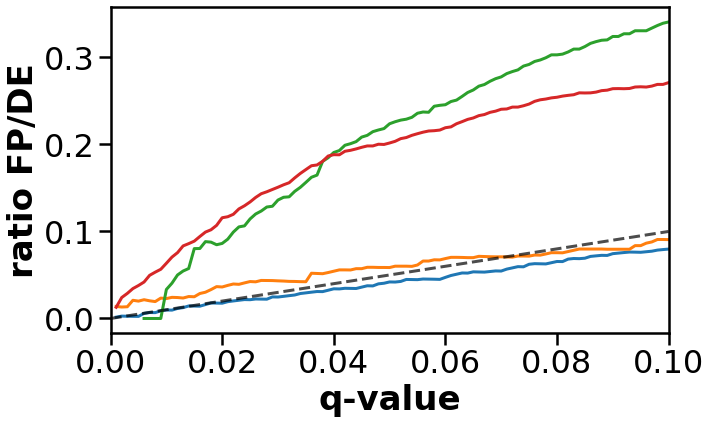
\includegraphics[width=0.5\linewidth]{../../result/report_plots/osw_FP_DE_all.png} & &%\includegraphics[width=0.3\linewidth]{} & 
        B 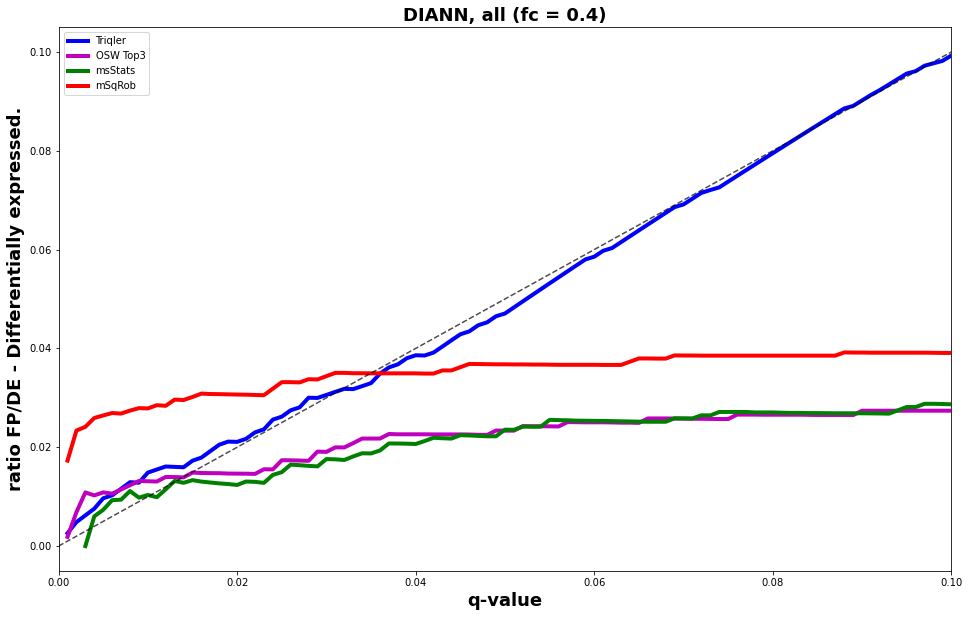
\includegraphics[width=0.5\linewidth]{../../result/report_plots/diann_FP_DE_all.png} & \\%\includegraphics[width=0.3\linewidth]{} \\ 
    \end{tabular}
  \caption{{\bf Comparison of calibration of the compared summarization methods.} We plotted the fraction of reported differentially abundant HeLa proteins as a function of $q$~value treshhold for (A) DDA generated spectral libraries and (B) DIA-Umpire geneated Pseudo spectra. The multiple test correction is performed with $q$~value for Triqler and Top3, while Benjamini-Hochberger [Add citation] is used for MSstats and MSqRobSum. \label{fig:frac_hela_vs_fdr}}
\end{figure}


\iffalse
\subsubsection*{Constant variance}

\begin{figure}[hbt]
    \centering
    %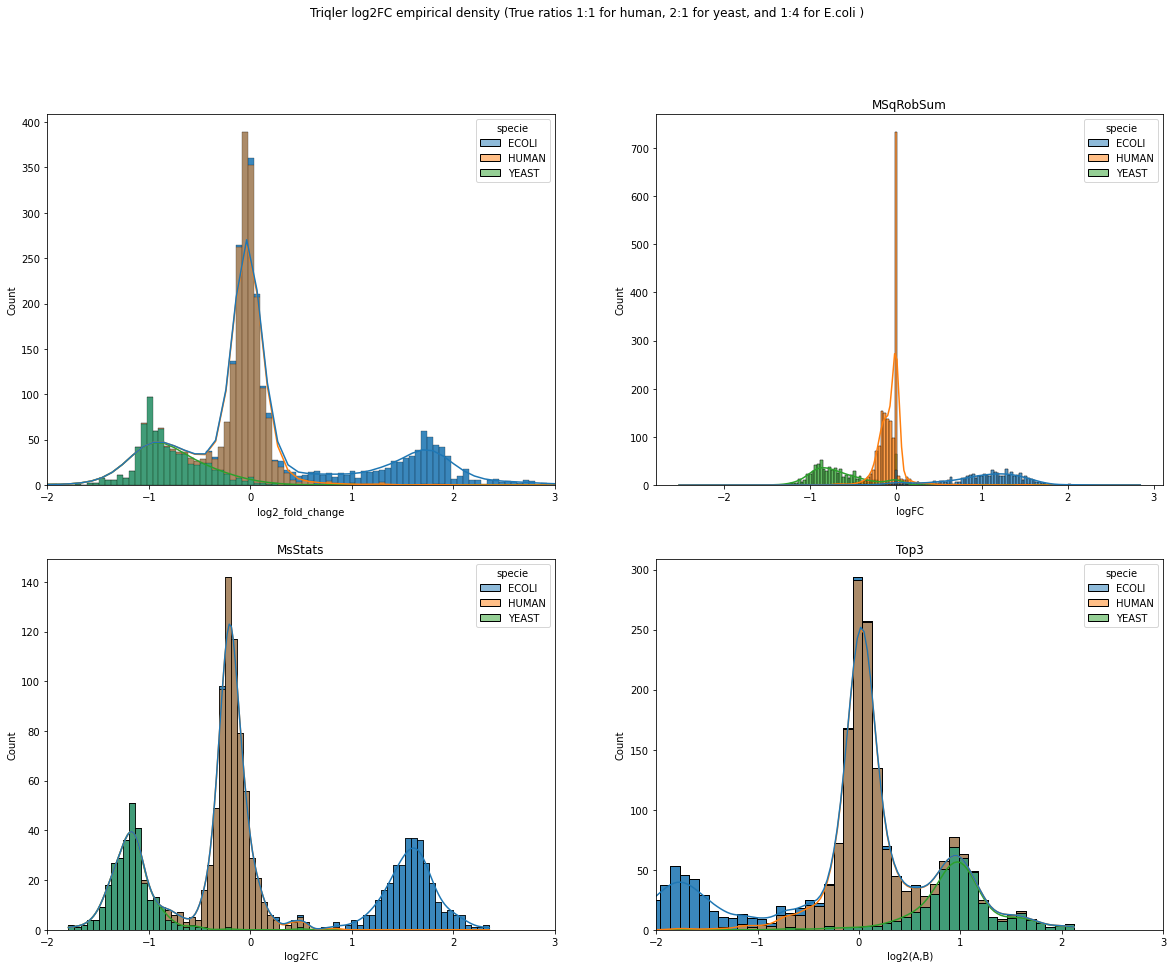
\includegraphics[width=16cm]{../../result/2021-08-13_docs_plots/intensity_plot.png}
    \begin{tabular}{lclc} 
        A  & &%\includegraphics[width=0.3\linewidth]{} & 
        E 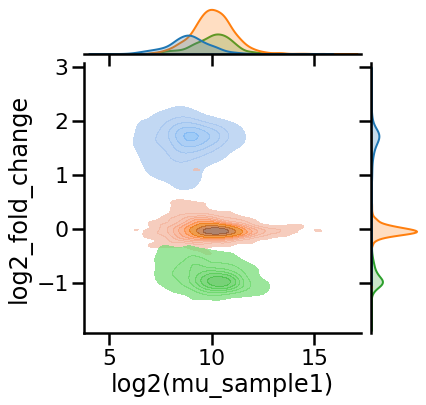
\includegraphics[width=0.35\linewidth]{../../result/report_plots/diann_scatter_triqler.png} & \\%\includegraphics[width=0.3\linewidth]{} \\ 
        B  & &%\includegraphics[width=0.3\linewidth]{} & 
        F 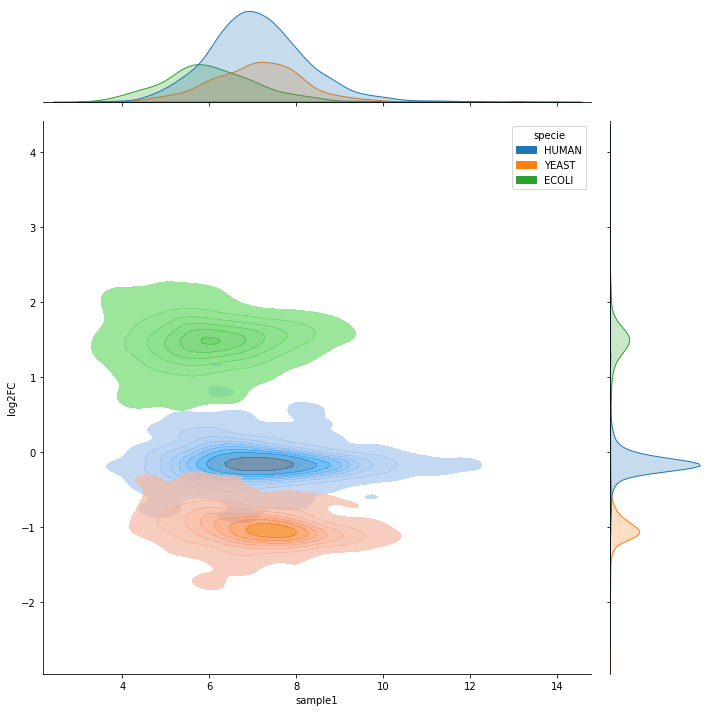
\includegraphics[width=0.35\linewidth]{../../result/report_plots/diann_scatter_msqrobsum.png} & \\%\includegraphics[width=0.3\linewidth]{} \\ 
        C  & &%\includegraphics[width=0.3\linewidth]{} & 
        G 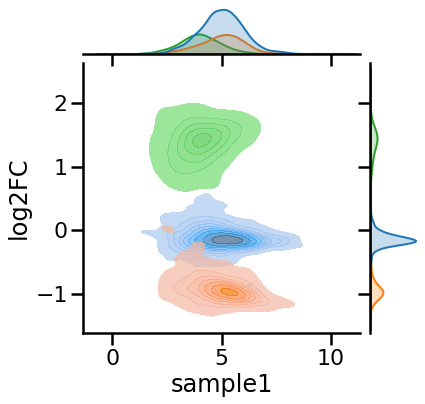
\includegraphics[width=0.35\linewidth]{../../result/report_plots/diann_scatter_msstats.png} & \\%\includegraphics[width=0.3\linewidth]{} \\ 
        D  & &%\includegraphics[width=0.3\linewidth]{} & 
        H 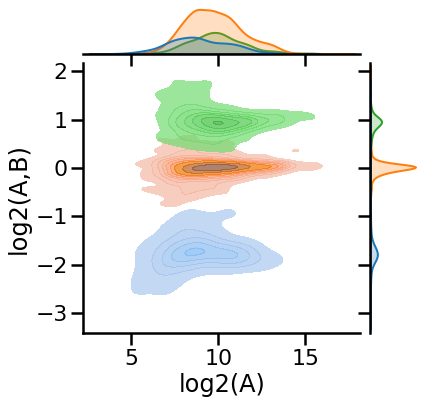
\includegraphics[width=0.35\linewidth]{../../result/report_plots/diann_scatter_top3.png} & %\includegraphics[width=0.3\linewidth]{} 
    \end{tabular}
    %\todo[inline]{Make scatter for OSW as well, and how to do with fig sizing?. Change the coloring and order of series so that they are coinsistent through the panels.}
    \caption{{\bf Comparison of reported fold change distributions.} We used peptide data from (A-D) Spectrum library matching and (E-H) pseudo spectra workflows as generated by 
    (A,E) Triqler, (B,F) MSqRobSum, (C,G) MSstats, and (D,H) Top-3. \label{fig:fc_histogram}}
\end{figure}
\fi


%\todo{Finish the truncated distribution fitting}

\begin{comment}
\subsection*{Protein quantification}

Log-transformed ratios (log2(A//B)) of proteins (humans proteins in orange, yeast proteins in green, and E. Coli proteins in blue) were plotted for each benchmarked software over the log-transformed intensity of sample A. The dashed horizontal line represents the expected log-fold change, while the fitted dashed line represents a linear regression for each species. Fig. \ref{fig:OSW_scatter} shows the results for OpenSwath and fig. \ref{fig:OSW_scatter} shows the results for DIA-NN. TOP3 and MsStat gives least biased results as protein intensities gets higher. Triqler gives the most biased results. 

\begin{figure}[H]
    \centering
    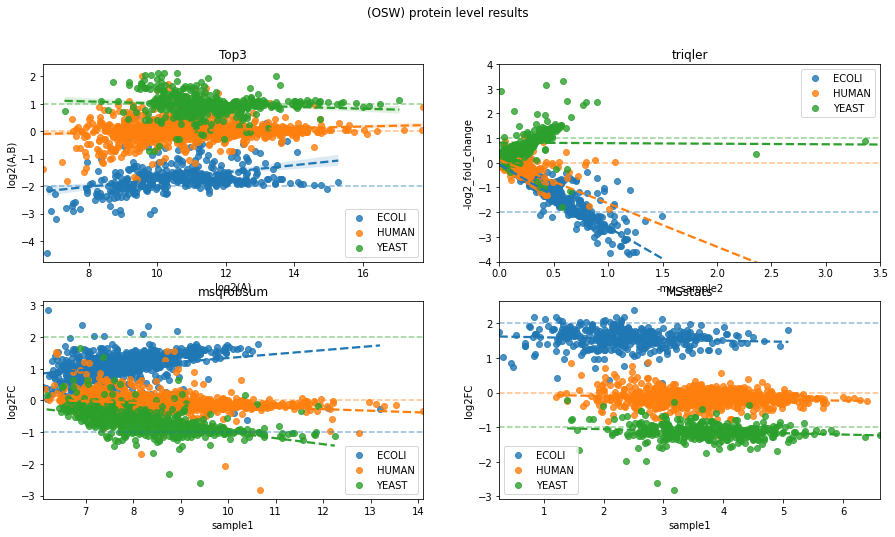
\includegraphics[width=16cm]{../../result/2021-08-13_docs_plots/OSW_protein_level_benchmark_scatter.png}
    \caption{OSW Protein level results from Triqler, Top3, MSstats and MSqRobSum.}
    \label{fig:OSW_scatter}
\end{figure}

\begin{figure}[H]
    \centering
    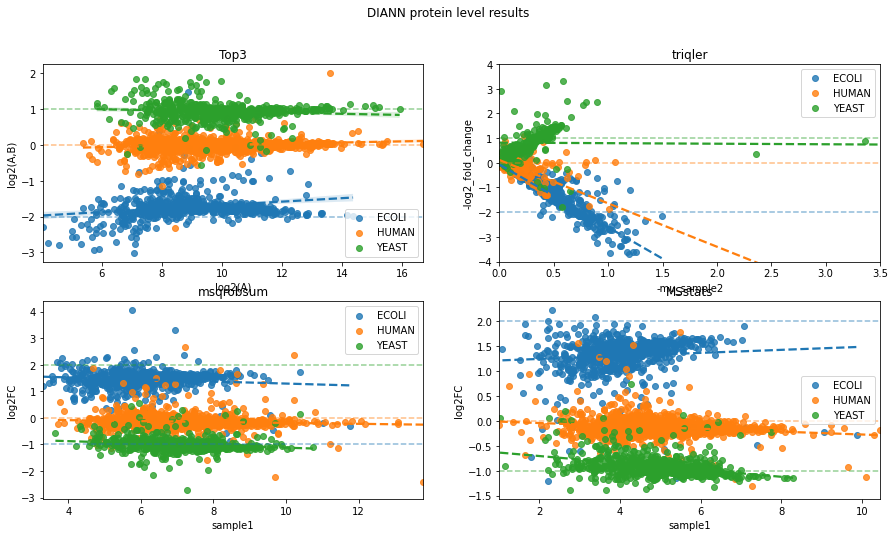
\includegraphics[width=16cm]{../../result/2021-08-13_docs_plots/DIANN_protein_level_benchmark_scatter.png}
    \caption{DIANN Protein level results from Triqler, Top3, MSstats and MSqRobSum.}
    \label{fig:OSW_scatter}
\end{figure}

Fig. \ref{fig:intensity_distribution} and \ref{fig:DIANN_intensity_distribution} show the protein quantity distributions with the different species; human (orange), E. Coli (blue), and yeast (green) highlighted in different colors for OSW \ref{fig:intensity_distribution} and DIA-NN \ref{fig:DIANN_intensity_distribution}. The human and yeast distribution apex is not centered at 0 in MsStats and MSqRob, while it is centered for triqler and top3. Likewise, the distribution for e.coli is closer to the true log2 fold change ratios for triqler and top3, while the apexes are skewed towards 0 for MsStats and MSqRob for both OSW and DIA-NN.     

\begin{figure}[H]
    \centering
    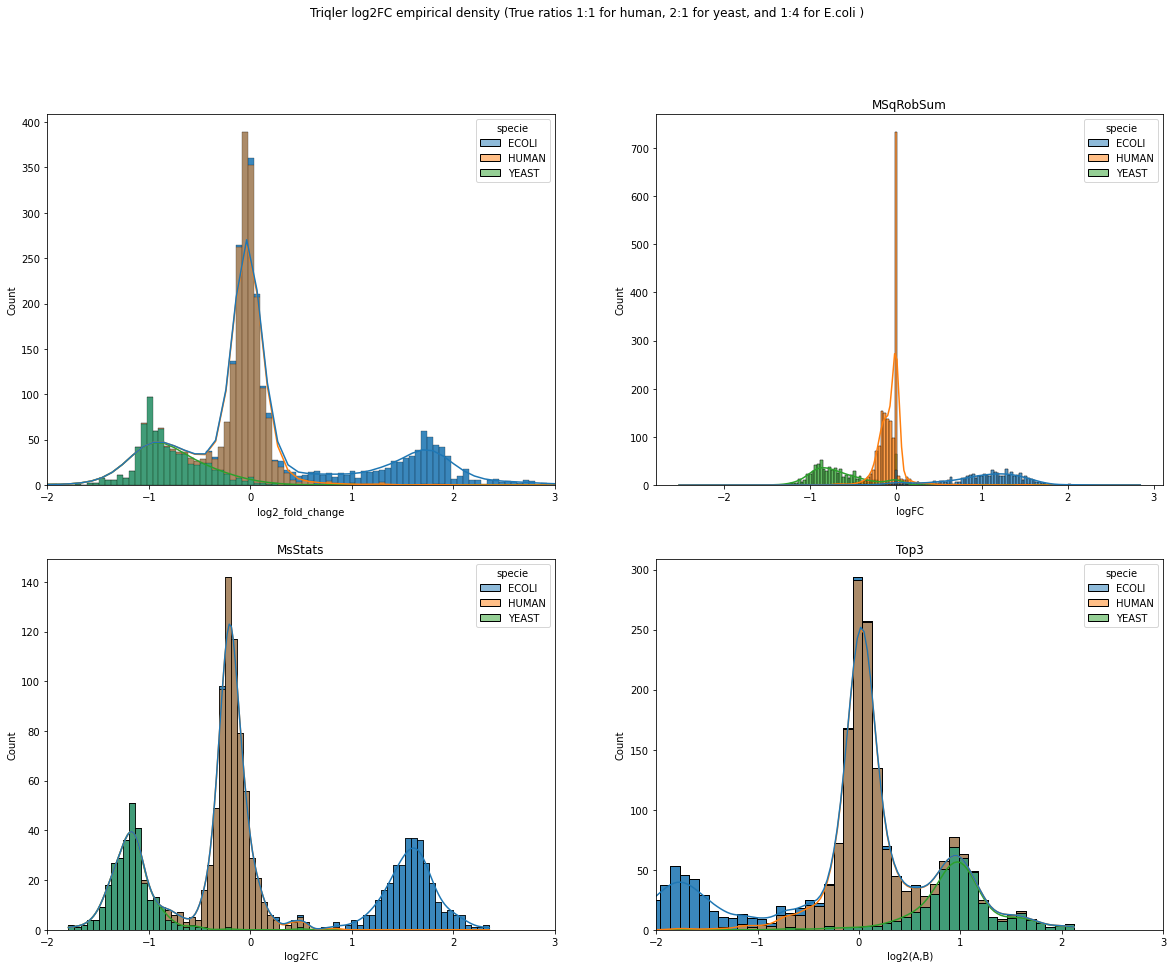
\includegraphics[width=16cm]{../../result/2021-08-13_docs_plots/intensity_plot.png}
    \caption{OSW Protein quantity distributions from Triqler, Top3, MSstats and MSqRobSum.}
    \label{fig:intensity_distribution}
\end{figure}

\begin{figure}[H]
    \centering
    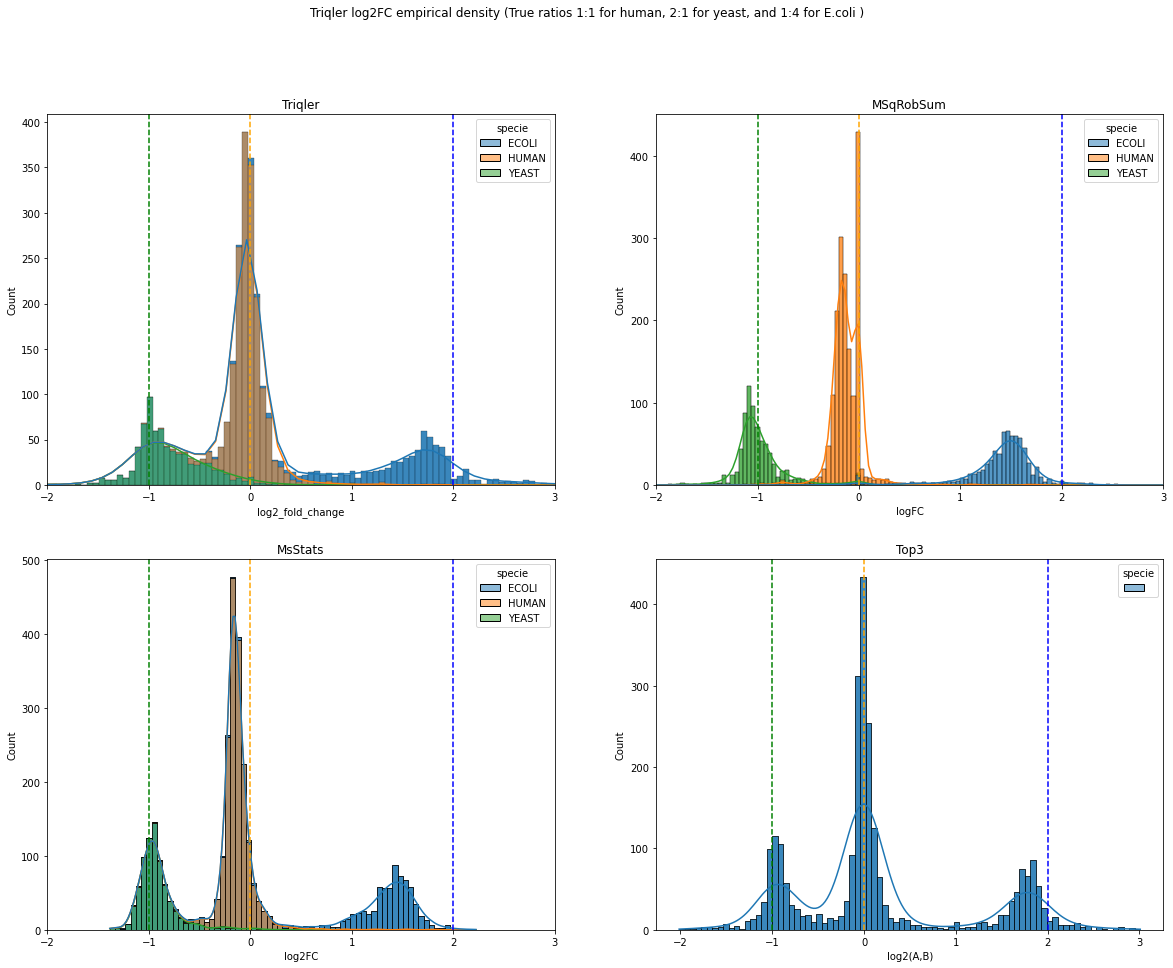
\includegraphics[width=16cm]{../../result/2021-08-13_docs_plots/DIANN_intensity_plot.png}
    \caption{DIANN Protein quantity distributions from Triqler, Top3, MSstats and MSqRobSum.}
    \label{fig:DIANN_intensity_distribution}
\end{figure}


Fig. \ref{fig:osw_n_diff_exp} and \ref{fig:DIANN_n_diff_exp} shows that the number of differentially abundance proteins is significantly higher for Triqler and MSqRobSum at different false discovery rates. MSqRobSum has a slightly higher number of differentially abundant proteins than triqler for OSW, and Triqler has slightly higher number of differentially abundant proteins for DIA-NN. The difference between the number of differentially abundant proteins are also smaller for MsStats and triqler and MSqRobSum for DIA-NN. 

\begin{figure}[H]
    \centering
    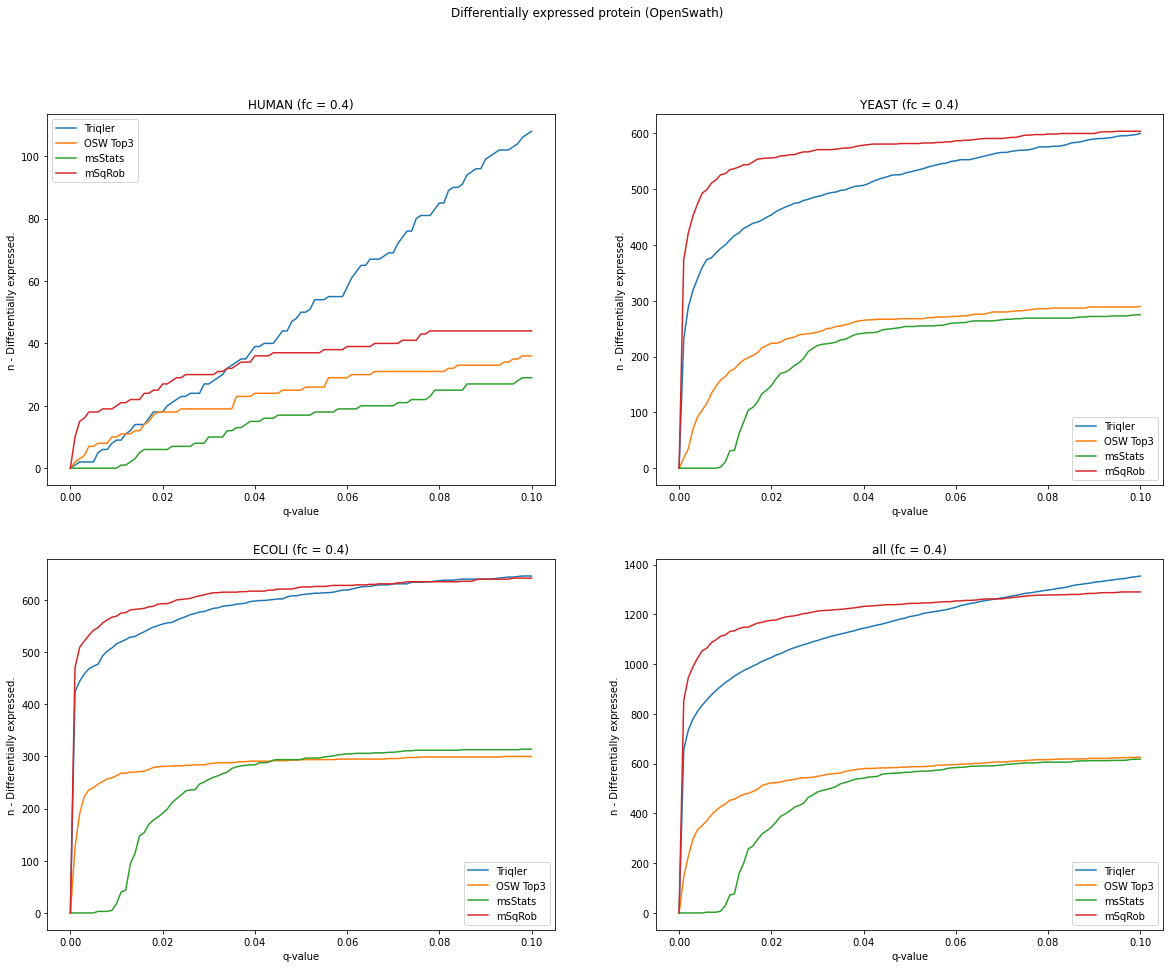
\includegraphics[width=16cm]{../../result/2021-08-13_docs_plots/n_diff_expressed.png}
    \caption{OSW Number of differentially abundant proteins for an OpenSwath analysis with triqler, top3, MsStats and MSqRobSum protein summarization.}
    \label{fig:osw_n_diff_exp}
\end{figure}

\begin{figure}[H]
    \centering
    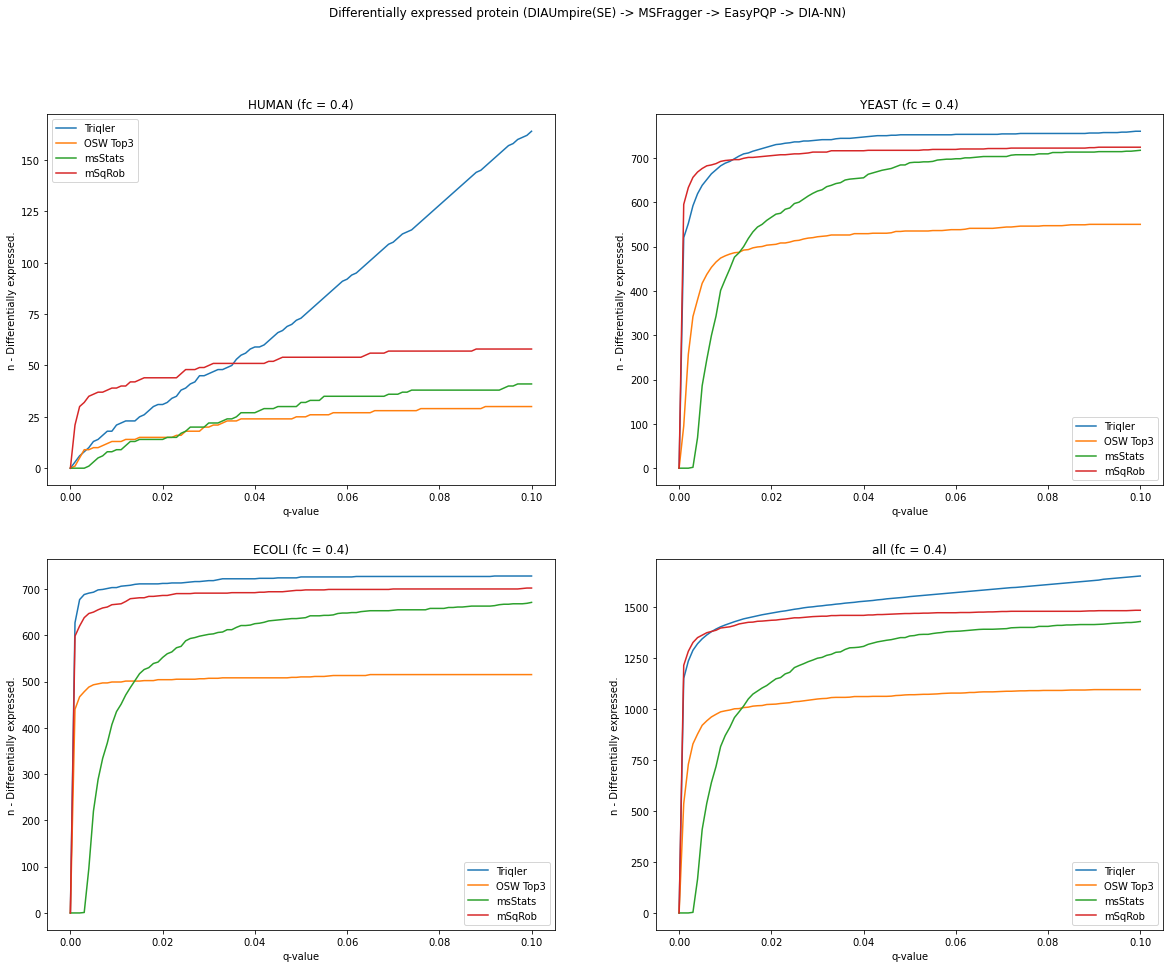
\includegraphics[width=16cm]{../../result/2021-08-13_docs_plots/DIANN_n_diff_expressed.png}
    \caption{DIANN Number of differentially abundant proteins for an OpenSwath analysis with triqler, top3, MsStats and MSqRobSum protein summarization.}
    \label{fig:DIANN_n_diff_exp}
\end{figure}



Fig. \ref{fig:osw_n_diff_exp} and \ref{fig:DIANN_n_diff_exp} shows that the ratio of false positives (human proteins) to the number of differentially abundant proteins for a given $q$~value level is more linear for triqler. At log2FC = 2 all methods are conservative at low $q$~values and anti-conservative at higher $q$~values. Triqler is better calibrated for low $q$~values and gets more conservative as the $q$~value threshold is increased. Top3, MsStats, and MSqRob are more conservative at low $q$~values and get less conservative as the $q$~value threshold increases.  

   
\begin{figure}[H]
    \centering
    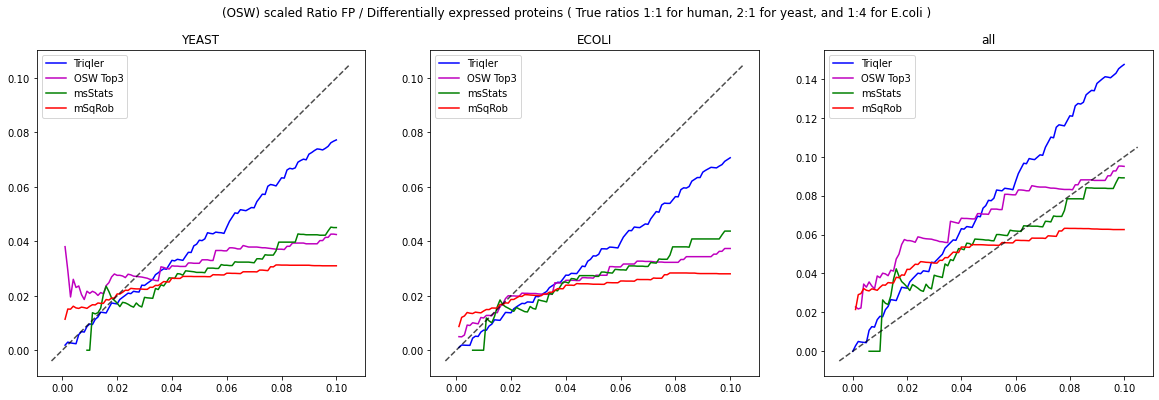
\includegraphics[width=16cm]{../../result/2021-08-13_docs_plots/calibration_plot_scaled.png}
    \caption{OSW $q$~value (x-axis) and false positive / number differentially abundant protein (y-axis) ratio.}
    \label{fig:osw_n_diff_exp}
\end{figure}

\begin{figure}[H]
    \centering
    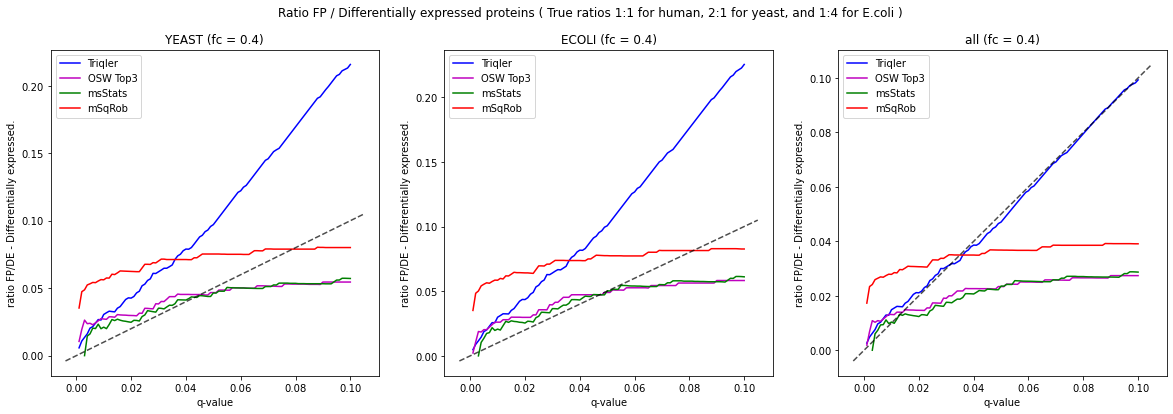
\includegraphics[width=16cm]{../../result/2021-08-13_docs_plots/DIANN_calibration_plot.png}
    \caption{DIANN $q$~value (x-axis) and false positive / number differentially abundant protein (y-axis) ratio.}
    \label{fig:DIANN_n_diff_exp}
\end{figure}

Fig. \ref{fig:osw_de_human_vs_de_specie} and \ref{fig:DIANN_de_human_vs_de_specie} shows  

\begin{figure}[H]
    \centering
    \includegraphics[width=12cm]{../../result/2021-08-13_docs_plots/de_human_vs_de_specie.png}
    \caption{OSW Number of differentially abundant humans (x-axis) and differentially abundant e.coli and yeast (y-axis).}
    \label{fig:osw_de_human_vs_de_specie}
\end{figure}

\begin{figure}[H]
    \centering
    \includegraphics[width=12cm]{../../result/2021-08-13_docs_plots/DIANN_de_human_vs_de_specie.png}
    \caption{DIANN Number of differentially abundant humans (x-axis) and differentially abundant e.coli and yeast (y-axis).}
    \label{fig:DIANN_de_human_vs_de_specie}
\end{figure}

\end{comment}


\section*{Discussion}

In bottom-up proteomics summarizing peptides to protein has been a long-established practice. There are several reasons protein summarization is beneficial. It gives lower variance among technical and biological replicates than peptide-level analysis, it reduces the amount of hypotheses tested and reduced the amount of missing values, which can have major impact on the quality of the analysis \cite{plubell2021can}.   

Here we have shown that Triqler operates well for DIA data, despite originally intended for DDA data. We also find that Triqler outperforms other protein summarization methods on our engineered benchmark set, both in terms of sensitivity and accuracy in its error estimates. Triqler is also able to detect significantly higher number of differentially abundant proteins for Yeast and E.Coli, while reporting low amount of differentially abundant HeLa proteins. 

One important remark is that the .FASTA database used to define the search space was truncated by keeping only one protein per peptide to control for any difference in protein inference strategies used in the protein summarization methods. There is currently no consensus in how to handle multiple proteoforms in bottom-up proteomics (Cite something from Humpty-Dumpty). Hence, we believe that protein inference strategies that can account for multiple proteoforms would greatly benefit the field by improving the quality of the quantitative analysis. 

We do see some differences in how DIA and DDA peptide-level abundance data appear. For instance there are more missing values in DDA than DIA data. However, we find that qualitatively the types of data are similar, at least in the sense that Triqler's underlying assumption of missing values seem to be as valid for DDA and DIA data.

Lastle, we want to highlight the benefit and importance as datasets such as the one provided by Navarro et al. \cite{navarro2016multicenter}. These benchmarking datasets make it easy for the scientific community to investigate computational tools by providing a golden standard and significantly reduces the treshold for benchmark studies. 





Key notes for the discussion:
\begin{itemize}
%  \item Why it is good with protein summarization (Humpty-Dumpty inspired argumentation).[X] 
%  \item Triqler is a good alternative for protein summarization. [X]
%  \item And this we have shown with the benchmark we conducted above. [X]
%  \item Summarize our findings from above. [X]
%  \item Discuss the protein inference problem. [X] 
%  \item Tell how we have performed our protein search on a truncated database for fair comparison.[X]
  %\item Highlight fair comparison. [X]
  \item Discuss future improvements.
%  \item Future improvement: Protein inference strategies which can account for multiple proteoforms. [X]
%  \item Discuss why dataset such as LFQ-bench is good (because it makes it easy to perform benchmarking and comparison).
  \item Add some more general notes about the field in general.
\end{itemize}



\section*{Acknowledgements}


\section*{Funding}

This work was supported by grants from the Swedish Research Council (grant 2017-04030) 

\section*{Supporting information}

\bibliographystyle{plain}
%\bibliography{benchmark}
\bibliography{benchmark.bib}
\end{document}



